%to have line numbers
%\RequirePackage{lineno}
\documentclass[10pt, letterpaper]{article}      
\usepackage[margin=.1cm,font=small,labelfont=bf]{caption}[2007/03/09]
%\usepackage{endnotes}
%\let\footnote=\endnote


\usepackage{setspace}
\usepackage{longtable}                        
\usepackage{anysize}                          
\usepackage{natbib}                           
%\bibpunct{(}{)}{,}{a}{,}{,}                   
\bibpunct{(}{)}{,}{a}{}{,}                   
\usepackage{amsmath}
\usepackage[% draft,
pdftex]{graphicx} %draft is a way to exclude figures                
%\usepackage{epstopdf}
\usepackage{hyperref}                             % For creating hyperlinks in cross references
 
% \usepackage[margins]{trackchanges}

% \note[editor]{The note}
% \annote[editor]{Text to annotate}{The note}
%    \add[editor]{Text to add}
% \remove[editor]{Text to remove}
% \change[editor]{Text to remove}{Text to add}

%TODO make it more standard before submission: \marginsize{2cm}{2cm}{1cm}{1cm}
\marginsize{2.5cm}{2.5cm}{.5cm}{.5cm}%{left}{right}{top}{bottom}   
					          % Helps LaTeX put figures where YOU want
 \renewcommand{\topfraction}{1}	                  % 90% of page top can be a float
 \renewcommand{\bottomfraction}{1}	          % 90% of page bottom can be a float
 \renewcommand{\textfraction}{0.0}	          % only 10% of page must to be text

 \usepackage{float}                               %latex will not complain to include float after float

\usepackage[table]{xcolor}                        %for table shading
\definecolor{gray90}{gray}{0.90}
\definecolor{orange}{RGB}{255,128,0}

\renewcommand\arraystretch{.9}                    %for spacing of arrays like tabular

%-------------------- my commands -----------------------------------------
\newenvironment{ig}[1]{
\begin{center}
 %\includegraphics[height=5.0in]{#1} 
 \includegraphics[height=3.3in]{#1} 
\end{center}}

 \newcommand{\cc}[1]{
\hspace{-.13in}$\bullet$\marginpar{\begin{spacing}{.6}\begin{footnotesize}\color{blue}{#1}\end{footnotesize}\end{spacing}}
\hspace{-.13in} }

%-------------------- END my commands -----------------------------------------



%-------------------- extra options -----------------------------------------

\usepackage{pdfpages} %load after xcolor, like at the end ideally i guess and
                      %turn off epstopdf


%%%%%%%%%%%%%
% footnotes %
%%%%%%%%%%%%%

%\long\def\symbolfootnote[#1]#2{\begingroup% %these can be used to make footnote  nonnumeric asterick, dagger etc
%\def\thefootnote{\fnsymbol{footnote}}\footnote[#1]{#2}\endgroup}	%see: http://help-csli.stanford.edu/tex/latex-footnotes.shtml

%%%%%%%%%%%
% spacing %
%%%%%%%%%%%

% \abovecaptionskip: space above caption
% \belowcaptionskip: space below caption
%\oddsidemargin 0cm
%\evensidemargin 0cm

%%%%%%%%%
% style %
%%%%%%%%%

%\pagestyle{myheadings}         % Option to put page headers
                               % Needed \documentclass[a4paper,twoside]{article}
%\markboth{{\small\it Politics and Life Satisfaction }}
%{{\small\it Adam Okulicz-Kozaryn} }

%\headsep 1.5cm
% \pagestyle{empty}			% no page numbers
% \parindent  15.mm			% indent paragraph by this much
% \parskip     2.mm			% space between paragraphs
% \mathindent 20.mm			% indent math equations by this much

%%%%%%%%%%%%%%%%%%
% extra packages %
%%%%%%%%%%%%%%%%%%

\usepackage{datetime}

%\usepackage{polski}
\usepackage[utf8]{inputenc}
% \usepackage[latin1]{inputenc}
\usepackage{tikz}
\usetikzlibrary{shapes,arrows,backgrounds}


%\usepackage{color}					% For creating coloured text and background
%\usepackage{float}
\usepackage{subfig}                                     % for combined figures

\renewcommand{\ss}[1]{{\colorbox{blue}{\bf \color{white}{#1}}}}
\newcommand{\ee}[1]{\endnote{\vspace{-.10in}\begin{spacing}{1.0}{\normalsize #1}\end{spacing}\vspace{.20in}}}
\newcommand{\emd}[1]{\ExecuteMetaData[/tmp/tex]{#1}} % grab numbers  from stata

%TODO before submitting comment this out to get 'regular fornt'
\usepackage{sectsty}
\allsectionsfont{\normalfont\sffamily}
\usepackage{sectsty}
\allsectionsfont{\normalfont\sffamily}
\renewcommand\familydefault{\sfdefault}

% \usepackage[margins]{trackchanges} (LM)
\usepackage{rotating}
\usepackage{catchfilebetweentags}

\usepackage{abstract}
\renewcommand{\abstractname}{}    % clear the title
\renewcommand{\absnamepos}{empty} % originally center
%-------------------- END extra options -----------------------------------------
\date{{}\today}
\title{  % remember to have Vistula University!!
Elderly Volunteering in Europe. Revisting Haski (2009) \footnote{This study was funded by grant \# 2016/21/B/HS4/03058 from
  Polish National Science Foundation (Narodowe Centrum Nauki).}
}
\author{
Leszek Morawski\thanks{EMAIL: ???@???
  \hfill I thank XXX.  All mistakes are mine.} \\
{\small Vistula University}
Adam Okulicz-Kozaryn\thanks{EMAIL: adam.okulicz.kozaryn@gmail.com
  \hfill I thank XXX.  All mistakes are mine.} \\
{\small Rutgers - Camden  and Vistula University}
}

\begin{document}

%%\setpagewiselinenumbers
%\modulolinenumbers[1]
%\linenumbers

\bibliographystyle{/home/aok/papers/root/tex/ecta}
\maketitle
\vspace{-.4in}
\begin{center}

\end{center}


\begin{abstract}
\noindent
\end{abstract}
\vspace{.15in} 
\noindent{\sc subjective wellbeing, volunteering, SHARE (Survey of Health, Ageing and Retirement in Europe) 
}
\vspace{.25in} 

\begin{spacing}{1.4} %TODO MAYBE before submission can make it like 2.0
\rowcolors{1}{white}{gray90}

%  instead \ExecuteMetaData[../out/tex]{ginipov} do \emd{ginipov}

% \begin{figure}[H]
%  \includegraphics[height=3in]{../out/gov_res_trust.pdf}\centering\label{gov_res_trust}
% \caption{woo}
% \end{figure}



%TODO !!!! have input here aok_var_des
%%%%%%%%%%%%%%%%%%%%%%%%%%%%%%%%%%%%%%%%%%%%%%%%%%%%%%%%%%%%%%%%%%%%%%%%%%%%%%

Rates of volunteering among the group of 50+ are much dispersed among countries. According to \citet{Oecd16} the rates range from above 30\% in the Netherlands, Irleand, Norwey, Switzerland to less than 10\% in Poland, Hungary, Greece, Portugal. Popularity of volunteering changes with age. In some countries, e.g., the Netherlands, France, Denmark and the UK, the volunteering rates for those in the group of 50+ are higher than for the groups of younger people. In other countries - Norway, Germany, Finland, Icleand, Switzerland  - the rates among elderly are higher than among the mid-age group (30-50) but they are lower than the rates for the group of 15-29. But there is also a group of European countries in which people 50+ are involved in  volunteering less often than younger people. These are the Central and East European countries (CEE) - Estonia, Latvia, Poland, Czech Republic, Lithuania, Hungary--and  Southern European countries (SEC)--Spain and Italy \citep{Oecd16}.  Age and volunteering may be related in different ways. It is possible that country specificity emobodied in its history and culture is signicant part of explanation of variaty in the volunteering rates. Presumably, the motives of elderly to be involved in volunteering are different from those of younger people \citep{wilson12}. \\

\textbf{Menchik and Weisbrod (1987)} propose to treat  volunteering either as an ordinary consumption good or as an investment good increasing an individual's income over time. \citet{haski09} noticed that elderly in comparison with young people are less motivated by carrer concerns and  more by social motive since volunteering give them  a  chance to participate in the usefull activities. In the "good conscience hypothesis" \textbf{(Freeman, 1997)} volunteering is something that people feel morally obligated to do when asked. This makes volunteering to be more like an obligation than a free personal choice that is rooted in an individual preferences. Altruistic volunteering  is more beneficial than volunteering resulting from social pressure. It is why we should expect weaker impact from it on subjective well-being if there are many volunteers around. Also, if there are many volunteering activites conducted,  some of them may have a limited value.  \\

There are demand and supply factors. The demand is mostly created by unmet demand for public goods and services. The supply depends on how people allocate their time to unpaid activities to improve their utility \citep{ziemek06}. This approach  suggests the positive relation between the degree of unsatisfactory supply of public good and services and the rates of formal volunteering. Inefficient markets and weak government are important determinants of formal volunteering popularity. This makes us to predict more volunteering in less developed countries where markets are inefficient and quality of government is low. However, this prediction seems to be false. For example, \textbf{Hank and Stuck (2008) and Siegrist and Wahrendorf (2009)}  clearly show higher rates in Northern European countries and lower rates in Eastern and Southern Europe. The same pattern appears in previously cited OECD data \citep{Oecd16} as well as in  \citet{Oecd15} that shows the rates of formal volunteering range from 57.3\% in Norway to 17.7\% in Czechia. Variation in the rates is larger if we concentrate on the volunteering among people aged 50 and over. They range from 37.9\% in the Netherlands to as little as 3.2\% in Poland. The lower rates in less developed countries suggest a considerable role of supply factors and transaction costs that may be are responsible for unmet demand for volunteering services. These transaction costs may include transport difficulties, lack of information, perceptions of volunteering and lack of variety in the opportunities. The low rates mean also that those who overcome all costs must have strong altruistic attitude toward volunteering. This make them significantly different from non-volunteers.  \\

The low rates in less developed countries are worrying since the demographic changes and financial distress in retirement sector  will touch elderly in a especially adverse way. Quality of life of elderly who are likely to experience negative life events due to health deterioration, reduction of income and smaller social contact network has become a major social issue. Volunteering may improve their QoL through engagement in a socially meaningful role and  gives meaning and purpose in life \textbf{(Greenfield and Marks, 2004; Prouteau and Wolff, 2008)}. The positive effect of volunteering on elderly are well known and commonly accepted, see:  \citet{morrow10}. Elderly seem to benefit more from volunteering than younger people \textbf{(Li and Ferraro, 2005; Van Willigen, 2000)}. \citet{jenkinson2013volunteering} surveyed forty experimental and cohort studies comparing the physical and mental health outcomes and mortality of a volunteering group to a non-volunteering group. They found that volunteering had favourable effects on depression, life satisfaction, wellbeing but not on physical health. Positive association between vounteering and subjective health was reported for example in  \citet{borgonovi08}, \cite{anderson14}, \cite{li06}, \cite{VanWilligen00}, \citet{detollenaere17}. \\ 

Helping others has positive effects on wellbeing. Those engaged in such activity report higher scores for subjective well-being \citep{haski09,morrow2003,thoits03,whillans2016}. \citep{meier08} showed that volunteering led to increased life satisfaction in a longitudinal study in Germany. \citet{wilson12} in his review essay on volunteerism research  listed the benefits of volunteering for a volunteer. The list included: enchancement in mental health and protection against symptoms of mentall illness, lower levels of morbidity and mortality, socioeconomic benefits such as increase in chances of obtaining a better education and a better job. Positive effect of volunteering was also found in a study based on 30 case studies from 11 European countries (\citet{ehlers11}). It was stressed that volunteering of elderly people help them to build new relationships with other volunteers but also with those whom they helped. According to findings presented in the study,  volunteering helps regain a meaningful activities after some adverse events.   \\

Volunteering is beneficial for society \citep{Oecd15,prouteau06}. It is considered to be a productive activity \citep{hank09}. This is important becouse demographic changes together with progress in health care increase time when elderly  are in relatively good health while being on retirement. This creates a stock of unused labor among elderly that may be effectively used with benefit for a volunteer and other members of a society.  This makes volunteering among elderly an intresting policy tool that may help to keep people in better health when they get older. The positive effect of volunteering has been recognized by many international organizations, too. In its 2001 recommendations the United Nations General Assembly identified volunteering as “an important component of any strategy aimed at poverty reduction, sustainable development, health, disaster prevention and overcoming social exclusion and discrimination” \textbf{(United Nations, 2001)}. In 2008, the European Parliament wrote about volunteering as “[the] most sustainable form of renewable energy” and encouraged Member States and regional and local authorities to “recognise [its] value in promoting social and economic cohesion” \textbf{(European Parliament, 2008)}. \\

Our study attempts to answer a question posed in \citet{morrow10}: "Under what conditions does volunteering enhance the well-being of older volunteers?" Our study is also similar to \citet{haski09}. \citet{haski09} included an extensive discussion of variations in volunteering rates according to main socio-economic variables such as age, gender and employment status among people  50+  in 12 Western and Southern European countries. Confirming other studies, \citet{haski09} found the highest rates of voluteering among elderly in Northern Europe and the lowest rates in Southern Europe. Apart from the confirmation of those previously discussed in the literature relations, the paper includes the discussion of variation in impact of volunteering on wellbeing among the european conutries. It was found that \textit{"in countries which encourage volunteerism and where volunteering is a social norm, such as in the Northern European countries, the relation of volunteering and wellbeing was rather small. At the same time in countries where voulnteering was not so popular  a correlation between volunteering and three indicators of well-being (health, depression, and chances for longer life) were rather strong."}  Our study is inspired by the above finding. Also, our results are related to a work by \citet{plagnol10} who claimed that "Individuals in countries with low rates of volunteering gain less from such activities–-in terms of well-being-–than those in countries with high rates of volunteering. We hypothesize: \\

\begin{enumerate}
\item H1: The effect of volunteering on SWB among elderly differs across countries.  
\item H2: The impact of volunteering on SWb depends on its level in a country. The relation between the impact and the popularity is either decreasing or the relation is convex (inverted U).
\end{enumerate}

Our analysis extends \citet{haski09} in a few directions. Firstly, she used data collected in 2005 and 2006 in the first wave of Survey of Health, Ageing and Retirement in Europe (SHARE). We use more current data collected in 2015 in the sixth wave of the SHARE survey. This allows us to include Central and Eastern European countries (CEE) into the analysis of volunteering among elderly that did not participated in the first wave of the SHARE survey. This extension is important since up to date the majority of the volunteering studies have been based on data from the United States or Western Europe \citep{casiday08}. This is unfortunate since remarkable different life courses of Western and Eastern Europeans should lead to new and interesting insights (\textbf{Sokolowski 2001}). \citet{plagnol10}, \citet{Oecd16} and \citet{Oecd15} show that the rates of formal volunteering in Eastern and Central Europe are significantly lower then in Western Europe. Inclusion of those countries gives us more variation while studing the relation between its popularity and QoL. Secondly, in the first wave of the SHARE survey volunteering had to be identified by a question on activities conducted during last 4 weeks preceeding the interview. From the wave 4, the respondents are asked about such activites during last 12 months. This change has made the rates of volunteering in the SHARE much closer to the rates published by the OECD. Third, we measure an association between volunteering and QoL by the Kendall tau-b correlation coefficient while \citet{haski09} used the Pearson correlations. We test the statistical significance of the differences between the correlation coefficients, which was not done in the previous study. We think that this step is important since some differences are small and it is not obvious if they are statistically meaningfull. Fourthly, We use the CASP-12 index as a measure of QoL among elderly. The CASP-12 is a shorter version of the CASP-19 that was created as a measure of quality of life (QoL) in older ages. The measure is based on the needs-satisfaction theory \textbf{(Maslow, 1943; Doyal and Gough, 1991)}. QoL using the CASP is assessed depending on the level of implementation needs in four areas relevant to the positive experience of older age: the possibility of influencing one's own  surroundings (Control), autonomous decision-making (Autonomy), self-realization and taking pleasure in	surroundings (Control), autonomous decision-making (Autonomy), self-realization and taking pleasure in  life (Pleasure) (\cite{hyde03}). Finally, we extend the descriptive statistical analysis by a regresion analysis to control for possible confounding factors. We are also intrested in identifying a selection effect into volunteering that can explain, at least, partly the relation found in the descriptive analysis.  

\section{Data}

We use data from the wave 6 of the Survey of Health, Ageing and Retirement in Europe (SHARE). The dataset provides wide range of information on the socio-economic status, health, and family relationships of people aged 50 or more in 18 European countries. The dataset includes information from 68,231 interviews (CAPI)\footnote{Computer-assisted personal interviewing.} conducted in 2015 in 18 countries - 11 countries were included in the wave 1 (Austria, Belgium, Denmark, France, Germany, Greece, Israel, Italy, Spain, Sweden, Switzerland) and 9 countries entered the survey later on (Czech Republic, Poland, Luxemburg,  Portugal, Slovenia, Estonia and Croatia). SHARE applies a concept of ex-ante harmonisation: there is one common generic questionnaire that is translated into the national languages using an internet based translation tool and processed automatically in a common CAPI instrument. In each participating country a probability sample was drawn. Due to different institutional conditions a uniform sampling design was impossible. For example, a simple random selection of households, from the central population register was used in in Denmark, while complex multistage design was applied in Greece. The  household level response rate ranged from 30.3\% in Luxemburg to 69.3\% in Greece \citep{bergmann17}. \\
In the paper we consider the formal volunteering that is conducted within a formal organisational structure, is self-governing, is not profit distributing and is independent of government. We do not consider the informal volunteering such as providing unpaid help to a friend or neighbour. The lengthy and detailed discussion of challenges associated with measuring volunteering can be found in \citet{salomon2017}. Volunteering is identified through respondent's answer to a question about activities done in 12 months preceeding the survey. We consider as a volunteer a person who gave a positive answer to a question: "Have you done any of these activities in the last month: Done voluntary or charity work."  Our definition of the volunteering is consistent with the UN\footnote{United Nations Volunteers Programme: Preparatory Committee for the Special Session of the General Assembly on the implementation of the outcome of the world summit for social development and further initiatives. Volunteering and social development. A/AC.253/16/Add.7. United Nations; 2000.} and the OECD approaches \citep{Oecd15,Oecd16}. The same measurment was previously used in \citet{haski09}. Comparison of different rates are presented in table \ref{Rates}. \\ 

%%% TABLE
\begin{spacing}{.9}
\begin{table}[H]
\centering 
\caption{Volunteering rates (\%). {\bf TODO:} spell out country names}  
\begin{small} 
	 {
\def\sym#1{\ifmmode^{#1}\else\(^{#1}\)\fi}
\begin{tabular}{l*{1}{ccc}}
\hline\hline
            &\multicolumn{3}{c}{(1)}               \\
            &\multicolumn{3}{c}{}                  \\
            &age50pshare1&age50pshare6&      age50p\\
\hline
AT          &    8.482871&    20.14157&    27.11111\\
BE          &    15.55375&     26.6472&      26.125\\
DK          &    17.68369&    31.42221&    23.88889\\
FR          &    14.23717&    22.86863&    28.33333\\
DE          &    10.77763&    23.85213&    25.44444\\
GR          &    3.101644&    7.022412&       4.625\\
IS          &     11.9421&    15.53073&    21.66667\\
IT          &    6.738869&    11.82818&    16.66667\\
NL          &    21.89474&           .&      37.375\\
SE          &    2.448454&    6.268717&          14\\
S           &    18.00267&    14.65221&    12.77778\\
CH          &     14.4958&    29.53292&        31.8\\
CZ          &           .&    8.876772&      12.125\\
PL          &           .&    3.428239&    9.222222\\
IR          &           .&           .&    36.88889\\
LU          &           .&    24.74916&    29.28571\\
HU          &           .&           .&       7.375\\
PT          &           .&    9.552845&    10.11111\\
SL          &           .&    12.15442&       30.25\\
EE          &           .&    8.756568&          14\\
Total       &    12.11328&    16.31088&    20.95359\\
\hline
\(N\)       &          20&            &            \\
\hline\hline
\end{tabular}
}

      \label{Rates} 
\end{small}
\end{table}
\end{spacing}
%%%% END: TABLE

The rates for the wave 1 are lower than those for the wave 5 and the wave 6. Ther is no much difference between the last two columns.  The rates for  the Central and East European countries are among the lowest ones.  Poland has rate below 4\%. The rates for Hungary, Estonia and Czech Republic are slightly bigger but they are below 9\%. Slovenia is the only country with the rate above 10\% among formery centrally-planned economies. The rates in Central and East European Countries (CEEs) are on levels similar to observed in Southern Europe - Greece (7\%), Spain (6\%), Italy (below 12\%), Portugal (below 10\%).  The country pattern observed in Table \ref{Rates} agrees with the results know previously in the literature. First of all, there is a large variation in rates. Secondly,  the highest rates are seen for  Northern and Western European countries - the Netherlands (close to 50\%), Denmark, Switzerland and Belgium (around 30\%) and the lowest rates in Eastern and Southern Europe. \\
The low rates in Southern and Eastern Europe may be partly due to tight family bonds in these countries and low welfare services. Elderly in Southern and Eastern European countries more often take care of grandchildren what limits their possibility to be involved in formal volunteerig \textbf{(Dykstra and Fokkema, 2011; Hank, 2007; Myck on grandfathers)}. Experience of  enforced volunteering  in former socialistic countries where people were required to devote their time for social, cultural and political causes may be another cause of low rates in Eastern Europe \textbf{(Kuti,2004; Anheier and Salamon, 1999, p.44).} The experience of forced volunteering  may lower the desire to provide assistance to others by making the “volunteering became obsolete” for the current elderly. On the other hand, the rates in some formerly socialistic countries--Czech Republic, Estonia or Slovenia--are currently higher than in Southern Europe. This makes us to speculate that historical reasons are not the main obstacles to low rates in those countries. Even if some people have unpleasant memories of volunteering in the past there are more general couses such as economic development that explain diversity in the rates of volunteering. We belive that an economic progress in Central and Eastern Europe that have been observed since the collapse of the communism may increase propenisty to volunteering among elderly. \\
Table \ref{CaspTtest} shows that the average levels of quality of life among volunteers are higher than among nonvolunteers in all countries. The highest values of casp are for volunteers in Denmark, Austria and Switzerland. The lowest values for non-volunteers in Greece, Portugal and Italy.


%%% TABLE
%\begin{spacing}{.9}
%\centering 
%\begin{scriptsize} 
%	 % matrix: caspTtest file: C:\projekty\NCN_AdamOK\wyniki\Papers\Paper2_Haski\tex\caspTtest.tex  14 Mar 2018 11:14:48
\begin{table}[htbp]
\caption{\label{clabel} Casp}\centering\medskip
\begin{tabular}{|l|c|c|c|c|}\hline  
 & 0  & 1  & b  & p  \\ \hline  
AT & 40.746261 & 42.304745 & -1.5584836 & 2.033e-12 \\ \hline 
BE & 39.679801 & 40.553373 & -.87357198 & 1.950e-07 \\ \hline 
DK & 42.030572 & 42.552391 & -.52181865 & .00052022 \\ \hline 
FR & 39.383067 & 40.455224 & -1.0721573 & 7.245e-07 \\ \hline 
DE & 40.010277 & 40.981818 & -.9715415 & 3.858e-08 \\ \hline 
GR & 33.224563 & 34.922481 & -1.6979181 & 1.119e-07 \\ \hline 
IS & 35.826884 & 37.928177 & -2.1012929 & 1.228e-06 \\ \hline 
IT & 36.379366 & 38.69181 & -2.3124442 & 6.025e-18 \\ \hline 
ES & 37.854395 & 39.69697 & -1.8425749 & 2.627e-08 \\ \hline 
S & 40.232082 & 40.777778 & -.54569587 & .01454333 \\ \hline 
CH & 41.272021 & 42.127219 & -.85519821 & 6.888e-06 \\ \hline 
CZ & 36.521263 & 37.411079 & -.88981543 & .00102886 \\ \hline 
PL & 38.20719 & 40.891304 & -2.6841142 & .00148375 \\ \hline 
LU & 40.815981 & 41.875399 & -1.0594187 & .00028108 \\ \hline 
PT & 35.387578 & 36.82 & -1.4324224 & .00403019 \\ \hline 
SL & 39.702349 & 40.778555 & -1.0762059 & .00001613 \\ \hline 
EE & 37.061064 & 39.706897 & -2.6458327 & 8.952e-19 \\ \hline 
  \end{tabular}
\end{table}

%      \label{CaspTtest} 
%\end{scriptsize}
%\end{spacing}
%%%%% END: TABLE


% W caspTtest \begin{table}[htp] zamien na \begin{table}[H]
\begin{table}[H]
\begin{minipage}[b]{0.56\linewidth}
\centering
\begin{spacing}{.9}
\centering 
\begin{scriptsize} 
	 % matrix: caspTtest file: C:\projekty\NCN_AdamOK\wyniki\Papers\Paper2_Haski\tex\caspTtest.tex  14 Mar 2018 11:14:48
\begin{table}[htbp]
\caption{\label{clabel} Casp}\centering\medskip
\begin{tabular}{|l|c|c|c|c|}\hline  
 & 0  & 1  & b  & p  \\ \hline  
AT & 40.746261 & 42.304745 & -1.5584836 & 2.033e-12 \\ \hline 
BE & 39.679801 & 40.553373 & -.87357198 & 1.950e-07 \\ \hline 
DK & 42.030572 & 42.552391 & -.52181865 & .00052022 \\ \hline 
FR & 39.383067 & 40.455224 & -1.0721573 & 7.245e-07 \\ \hline 
DE & 40.010277 & 40.981818 & -.9715415 & 3.858e-08 \\ \hline 
GR & 33.224563 & 34.922481 & -1.6979181 & 1.119e-07 \\ \hline 
IS & 35.826884 & 37.928177 & -2.1012929 & 1.228e-06 \\ \hline 
IT & 36.379366 & 38.69181 & -2.3124442 & 6.025e-18 \\ \hline 
ES & 37.854395 & 39.69697 & -1.8425749 & 2.627e-08 \\ \hline 
S & 40.232082 & 40.777778 & -.54569587 & .01454333 \\ \hline 
CH & 41.272021 & 42.127219 & -.85519821 & 6.888e-06 \\ \hline 
CZ & 36.521263 & 37.411079 & -.88981543 & .00102886 \\ \hline 
PL & 38.20719 & 40.891304 & -2.6841142 & .00148375 \\ \hline 
LU & 40.815981 & 41.875399 & -1.0594187 & .00028108 \\ \hline 
PT & 35.387578 & 36.82 & -1.4324224 & .00403019 \\ \hline 
SL & 39.702349 & 40.778555 & -1.0762059 & .00001613 \\ \hline 
EE & 37.061064 & 39.706897 & -2.6458327 & 8.952e-19 \\ \hline 
  \end{tabular}
\end{table}

      \label{CaspTtest} 
\end{scriptsize}
\end{spacing}
    \label{table:student}
\end{minipage}\hfill
\begin{minipage}[b]{0.4\linewidth}
\centering
\captionof{figure}{Change in quality of life v volunteering rate. {\bf TODO:} on y axix say that differemce is volunteers-non-volunteers}
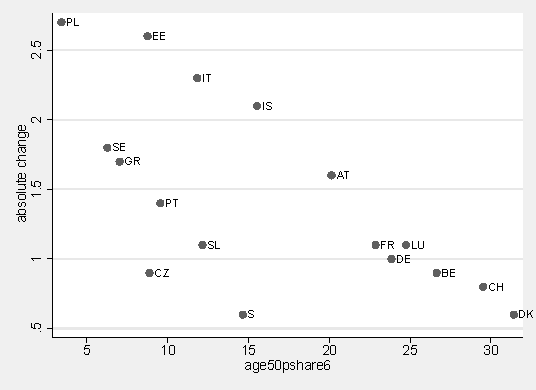
\includegraphics[height=2.5in]{abs_casp.pdf}
% \captionof{figure}{Change in quality of life}
\label{fig:casp}
\end{minipage}
\end{table}


The means in Eastern European countries (Poland, Estonia, Czech Republic) are higher than in Southern European for both volunteers and non-voluteers. The distributions of casp for volunteers and nonvolunteers show higher concentration of large values among volunteers (see Appendix). The differences in the means decrease for the countries with higher volunteering rate.  The differences in  Denmark, Switzerland, Belgium and Germany are less then 1.0. In countries where the rates are low the differences are above 1.5 - in Poland it is 2.7, in Spain 1.8, in Greece 1.7 and in Estonia 2.6. The negative relation suggests that "more volunteers in a country makes smaller increase in a volunteer wellbeing." 

Figure \ref{fig:casp} shows bigger heterogenity of the rates among the low rate countries. In Czech Republic, Portugal and Estonia the rates are similar but the absolute differences in the means are significantly different. At the same time the rates in Czech Republic and Slovenia are lower than in France, Germany, Luxemburg but the differences in means are at similar levels in all these countries. This comparison suggests that the large rates are associated with smaller impact on wellbeing what is consistent with findings in \citet{haski09} and \citet{plagnol10}. It seems that country specific factors do not play significant role among those countries. Regardless of  the rate, the impact of volunteering on average QoL is the same. Larger heteregenity  among the low rate countries suggests bigger role of country specific factors. Low popularity of volunteering is associated with large range of differences in casp. The possible explanation is that in highly developed countries formal volunteering is well organized with the efficient help from governmant but many tasks done by volunteers are not of high importance. In less developed countries there more barriers to volunteering,  which lowers supply of volunteers but the performed tasks are truly relevant. This makes volunteers to have strong feelings of being involved in necessary and highly valued activities. However, it does not explain why there is so large heterogenity among the low rate countries.   

%\textbf{health} \\
%We use similar measure of subjective health to the one used in Haski(2009). This is the self-perceived health variable with the respondents that range from "very bad" to "very good". Subjective health is also higer in more developed countries. In this case people from Southern European countries repored on average highher levels than those from Eastern Europe. The lowes mean values were found for Poland, Estonia, Croatia, Slovenia, Czech Rep. and in Portugal.


\section{Results}

We use the Kendall's tau-b correlation coefficient to describe the association between the the quality of life index (casp) and involvment in volunteering. The Kendall's correlation coefficient is appriopriate for either ordinal or interval data. This makes it the better measure than the Pearson correlation coefficient that may be used only for interval data.  Also, the Pearson coefficient is a measure of the linear correlation between two variables, which is not an attractive property in our case. Additionally, the Kendall's tau is less sensitive to outliers  \citet{khamis08}. The Kendall's correlation coefficients range from 15.4\% (Isreal) to 3.3\% (Sweden) suggesting a non-linear association between volunteering and QoL. The values of Kendall's tau-b correlation coefficients and the Pearson correlations coefficients from \citet{haski09} are compared below in figure \ref{fig:taub}.


\begin{figure}[H]
\centering
\caption{Correlations of volunteering and subjective wellbeing.  \textbf{popraw format}} 
\label{fig:taub}
\begin{minipage}{1\linewidth}
\subfloat[Life satisfaction (\citet{haski09})]{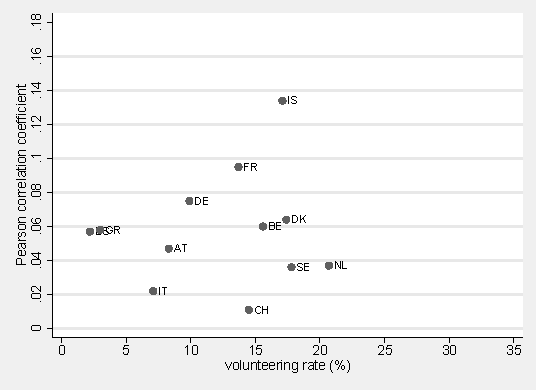
\includegraphics[height=2.7in]{Haski_lifesat.pdf}}\quad
\subfloat[Quality of life (casp)]{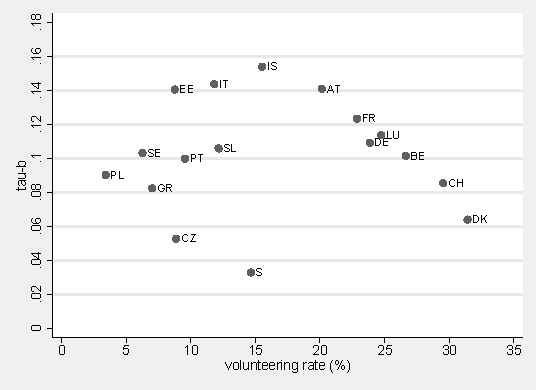
\includegraphics[height=2.7in]{Kendall_casp.pdf}}~\\
{\footnotesize Notes: (a) wave 1 (2006-2007), (b) wave 6 (2015) }~\\
{\footnotesize Source: \citet{haski09} [Table 3] and own calculations based on SHARE Wave 6.}
\end{minipage}
\end{figure} 

%
%\begin{figure}[H]
% 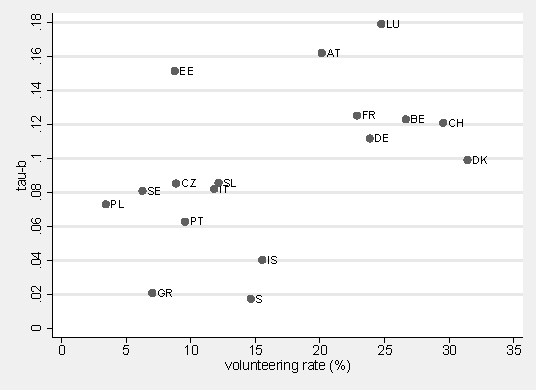
\includegraphics[height=3in]{Kendall_h.pdf}
% \centering
% \label{fig:tauH}
%\caption{tau subjective health}
%\end{figure}


 The significance tests confirm concave relation between the effect of volunteering on QoL and values of the volunteering rate. The p-values for the tests are given in the Appndix.  The point estimate for tau-b for Germany (0.109) is not statistically different from the estimate for Slovenia (0.106), Spain, Belgium, Portugal, Poland, Switzerland, Croatia and Greece (0.082). This homogenous group in dimension of the impact is highly heterogenous in dimension of the rate of volunteering. At the same time the tau-b for Estonia (0.141) is statistically different from the tau-b estimates in Slovenia (0.106), Poland(0.090) and Czech Republic (0.053) but  is the same as in France, Luxemburg and Austria. The tests confirm the finding in \citet{haski09} about non-linear pattern of associations between  the rate of volunteering and its impact on wellbeing. Figure \ref{fig:taub} shows that our approach based on the tau-b measure and casp index makes that finding even more convincing. \citet{haski09} discussed two explanations regarding concavity of the realtion betweem the volunteering rate and its impact on wellbeing. The first one stresses differences in motives for volunteering according to the economic developmnent of a country. In highly developed countries with the strong welfare system volunteering is a part of a social norm and it is not always related to solving real problems. In less developed countries with weaker welfare state, people are involved in volunteering only becouse of their altruistic preferences without feeling any social pressure. That is why they more often feel the sense of fullfilment  The second explanation is based on the Social Origins Theory \textbf{(Salamon and Anheier 1998)}. This argument states that the state through its genorouse social welfare policy satisfies demand for most social needs efficiently constraining supply of volunteering by non-govermental organizations. This crowding out effect does not exist in countries with less genorouse social welfare policy. In those countries volunteers are usually involved in solving the important social problems what increases their subjective wellbeing. Both arguments help to understand why volunteering can have a limited impact on wellbeing in reach countries. However, they do not explain why that impact may also be low in less developed countries. \textbf{[AOK: something is missing here. It would be nice to have some discussion on reasons why the association may be low when the rate is low. Any idea ? for some general ideas see commit message]} \\

However, it is possible that the low associations observed in these countries are due to selection into volunteering people who \textbf{[i tak sa zadowolni, nawet bez wolonariatu]}. Table 3 presents descriptive statistics for volunteers and non-volunteers together with the significance tests for the differences in means.  \\

{\bf TODO:} explain that 0 nonvolunteers and 1 volunteers
% POdzielić kraje na CEE, SE i WE
%%% TABLE
\begin{spacing}{.9}
\centering 
\begin{tiny} 
	 % matrix: Desc0 file: C:\projekty\NCN_AdamOK\wyniki\Papers\Paper2_Haski\tex\descTtest0.tex   9 May 2018 13:36:35
\begin{table}[htbp]
\caption{\label{clabel} Descriptive statistics}\centering\medskip
\begin{tabular}{lccccccccccccccc} \hline \hline
 & edu0  & edu1  & p  & age0  & age1  & p  & sex0  & sex1  & p  & h0  & h1  & p  & inc0  & inc1  & p  \\  \hline 
AT &       9.2 &      10.3 &       0.0 &      67.6 &      67.1 &      28.4 &      56.5 &      56.8 &      89.3 &      26.2 &      14.3 &       0.0 &      42.8 &      45.6 &      16.8 \\  
BE &      12.5 &      13.4 &       0.0 &      65.2 &      64.6 &       5.6 &      51.1 &      49.1 &      23.9 &      18.1 &      12.8 &       0.0 &      48.6 &      50.3 &      26.0 \\  
DK &      13.4 &      14.1 &       0.0 &      64.9 &      64.4 &      25.3 &      51.6 &      52.2 &      78.0 &      18.0 &      12.0 &       0.0 &      91.8 &      91.7 &      97.8 \\  
FR &      11.7 &      13.3 &       0.0 &      66.4 &      65.6 &       4.1 &      53.2 &      49.2 &       7.2 &      28.4 &      19.1 &       0.0 &      40.7 &      43.6 &      10.5 \\  
DE &      12.7 &      13.8 &       0.0 &      65.8 &      65.1 &       6.4 &      51.2 &      47.0 &       3.1 &      33.4 &      28.5 &       0.6 &      44.1 &      48.2 &       0.4 \\  
S &      11.8 &      12.3 &       0.6 &      69.0 &      69.8 &       4.4 &      50.6 &      57.1 &       0.9 &      20.1 &      20.0 &      95.0 &      48.5 &      45.7 &       0.9 \\  
CH &       8.7 &       9.3 &       0.7 &      67.7 &      67.0 &       7.8 &      54.0 &      51.4 &      25.2 &      16.1 &       7.2 &       0.0 &     107.2 &     115.4 &       4.9 \\  
GR &      10.0 &      10.6 &       2.9 &      65.5 &      64.7 &      16.7 &      50.2 &      68.3 &       0.0 &      21.5 &      22.8 &      62.8 &      24.8 &      22.0 &      16.3 \\  
IS &      12.8 &      14.6 &       0.0 &      67.1 &      68.2 &       7.7 &      54.0 &      56.2 &      57.2 &      22.2 &      25.8 &      28.1 &      33.5 &      39.2 &       0.2 \\  
PT &       6.7 &       9.2 &       0.0 &      65.8 &      65.6 &      80.0 &      44.9 &      53.5 &      10.1 &      56.4 &      49.5 &      19.0 &      18.6 &      21.0 &      26.6 \\  
IT &       9.4 &      10.8 &       0.0 &      65.7 &      64.8 &       5.5 &      48.4 &      54.5 &       1.4 &      30.7 &      22.1 &       0.0 &      26.7 &      29.8 &       0.0 \\  
ES &       9.3 &      12.2 &       0.0 &      67.4 &      65.8 &       0.8 &      50.0 &      56.8 &       3.5 &      26.3 &      17.3 &       0.1 &      22.5 &      27.4 &       0.0 \\  
CZ &      12.4 &      13.7 &       0.0 &      67.0 &      67.7 &      10.8 &      56.9 &      60.5 &      19.9 &      38.8 &      29.9 &       0.1 &       6.9 &       7.3 &      11.6 \\  
PL &      10.6 &      13.2 &       0.0 &      64.1 &      61.2 &       2.0 &      50.2 &      56.5 &      40.1 &      42.0 &      26.1 &       3.1 &       9.3 &      10.1 &      63.7 \\  
SL &      10.8 &      11.8 &       0.0 &      66.0 &      63.9 &       0.0 &      54.2 &      52.4 &      47.5 &      32.0 &      27.7 &       7.4 &      18.3 &      19.0 &      43.3 \\  
EE &      12.0 &      14.0 &       0.0 &      66.9 &      63.3 &       0.0 &      59.1 &      61.9 &      29.7 &      65.7 &      44.9 &       0.0 &       7.9 &       9.6 &       0.0 \\  
\hline \hline \end{tabular}
\end{table}

      \label{DescT0} 
\end{tiny}
\end{spacing}
%%%% END: TABLE

Both groups are different in their socio-economic characteristics. In all countries volunteers have better formal education (higher average number of years of education). Everywhere the shares of people with tertiary education are higher among volunteers, while the shares of people with primary education are lower. In countries with low volunteering the differences in a education structure are larger. In Poland the ratio of a share of people with a tertiary  education among volunteers over a share of such people among non-volunteers is 3.49. The respective ratios for Spain, Czech Republic, Estonia are: 2.77, 2.29 and 1.99, while for for Denmark it is 1.23, for Belgium 1.45, and for Switzerland it is 1.54. 

Differences in average age vary across countries. The means are  not statistically different  in Austria and in Denmark among Western European countries. In other countries from that group volunteers are younger  on average than non-volunteers. The exception is Sweden where volunteers are older. The histograms reveal in Belgium, Denmark, France, Germany,Switzerland and Luxemberg there are noticebly larger shares of volunteers in the age group of 65-70. In Greece and Portugal average ages in both gropus are not statistically different. In Isreal volunteers are older while in Spain and Italy they are younger on average than non-volunteers. In Czech Republic the averages are not significantly different while in Poland, Estonia and Slovenia volunteers are younger. The differences in average age in these countries are above 2 years what seems to be larger differences than in countries from other groups. In Poland and Estonia there are larger shares of people in the age group 50-55 among volunteers.  In Slovenia the difference is due to smaller share of volunteers older then 70 years. \textbf{[Comment ?]}

In many countries the shares of women and men among volunteers and non-volunteers are the same. In France and Germany there are more males involved in voluntering while in Switzerland the share of women among volunteers is larger. In Grecee, Italy and Spain women are more often involved in volunteering than man. There are no gender effect on volunteering in the CEE countries.Volunteers have better subjective health.  In Table \ref{DescT0} we found that smaller fraction of volunteers declare at most fair subjective health. Only in Switzerland, Greece, Isreal and in Portugal the fractions are the same.  Our measure of income takes into account differences in purchesing power parities and economy of scale due to a number of people living in a household. We apply the modifed OECD scale to control for decreasing living cost per person. We find no clear pattern between average income and volunteering. The differences in means are signifcant for Germany, Sweden, Switzerland, Luxemburg, Isreal, Italy and Estonia. In all countries except Sweden average income among volunteers were higher than among non-volunteers. Conditional distributions of equivalized income (Appendix) present a much richer picture. In all Southern and Eastern European countries there are more people with high income among volunteers than among non-volunteers. In  Western Europe, it is observed only for  Austria, Belgium, France, Germany. Sweden presents a unique case - there are more people with low income among volunteers. The distributions for Germany and Luxemburg reveal another interesting phenomenon. Namely, there is a small group of very rich people among non-volunteers that does not exist among volunteers.

Volunteers and volunteers differ according to socio-economic characteristics. Simple logit models confirm this. For each country education is significant variable explaining selection into volunteering. In majority of countries there is a selection according to age and subjective health, also. 

\subsubsection{Determinants of volunteering}



%%%%%%%%%%%%%%%%%%  LOGIT %%%%%%%%%%%%%%%%%%%%%%%%%

%%% TABLE
\begin{spacing}{.9}
\begin{table}[H]
\centering 
\caption{Logit: volunteering [CEE (Central and East European) and SE (South European) countries].}  
\begin{small} 
	 {
\def\sym#1{\ifmmode^{#1}\else\(^{#1}\)\fi}
\begin{tabular}{l*{10}{c}}
\hline\hline
            &\multicolumn{1}{c}{All}&\multicolumn{1}{c}{GR}&\multicolumn{1}{c}{IS}&\multicolumn{1}{c}{PT}&\multicolumn{1}{c}{IT}&\multicolumn{1}{c}{ES}&\multicolumn{1}{c}{CZ}&\multicolumn{1}{c}{PL}&\multicolumn{1}{c}{SL}&\multicolumn{1}{c}{EE}\\
\hline
vol         &               &               &               &               &               &               &               &               &               &               \\
gdp         &       1,060***&               &               &               &               &               &               &               &               &               \\
gdp2        &       1,000***&               &               &               &               &               &               &               &               &               \\
age: 60-70  &       1,114** &       0,968   &       1,594+  &       1,135   &       1,527** &       1,324   &       1,101   &       1,088   &       0,899   &       0,756+  \\
age: 71+    &       1,007   &       0,837   &       1,769*  &       0,896   &       1,407*  &       1,320   &       1,522*  &       1,314   &       0,645** &       0,721+  \\
0b.female   &       1,000   &       1,000   &       1,000   &       1,000   &       1,000   &       1,000   &       1,000   &       1,000   &       1,000   &       1,000   \\
1.female    &       1,068*  &       2,158***&       1,159   &       1,271   &       1,311** &       1,405*  &       1,230+  &       1,377   &       0,971   &       0,990   \\
1b.isced1   &       1,000   &       1,000   &       1,000   &       1,000   &       1,000   &       1,000   &       1,000   &       1,000   &       1,000   &       1,000   \\
2.isced1    &       1,523***&       1,378   &       1,608   &       4,080***&       1,560** &       1,622*  &       1,314   &               &       1,870+  &       4,159   \\
3.isced1    &       2,123***&       1,160   &       2,328** &       2,609*  &       2,255***&       3,727***&       2,301** &       4,840*  &       2,698** &       5,451+  \\
4.isced1    &       3,241***&       1,863***&       3,404***&       3,446***&       1,858** &       4,995***&       4,892***&      17,902***&       4,165***&      11,992*  \\
0b.sphusPlus&       1,000   &       1,000   &       1,000   &       1,000   &       1,000   &       1,000   &       1,000   &       1,000   &       1,000   &       1,000   \\
100.sphusPlus&       1,138***&       1,211   &       1,109   &       1,392   &       0,960   &       0,927   &       1,514** &       0,646   &       1,012   &       1,621** \\
0b.sphusMinus&       1,000   &       1,000   &       1,000   &       1,000   &       1,000   &       1,000   &       1,000   &       1,000   &       1,000   &       1,000   \\
100.sphusMinus&       0,811***&       1,262   &       1,470+  &       1,052   &       0,684** &       0,720+  &       0,864   &       0,613   &       0,991   &       0,719*  \\
income      &       1,001***&       0,997   &       1,010** &       0,999   &       1,015** &       1,008** &       1,007   &       0,999   &       1,000   &       1,060***\\
1b.hhsize1  &       1,000   &       1,000   &       1,000   &       1,000   &       1,000   &       1,000   &       1,000   &       1,000   &       1,000   &       1,000   \\
2.hhsize1   &       0,931*  &       0,822   &       0,824   &       0,788   &       0,745+  &       0,633*  &       0,764+  &       0,681   &       1,061   &       0,551***\\
3.hhsize1   &       0,909*  &       0,850   &       0,910   &       0,806   &       0,810   &       0,596*  &       0,630*  &       0,335+  &       1,230   &       0,588*  \\
4.hhsize1   &       0,846** &       0,450** &       1,213   &       0,488   &       0,521** &       0,461*  &       1,069   &       0,768   &       1,224   &       0,688   \\
5.hhsize1   &       0,956   &       1,307   &       1,642   &               &       0,685   &       0,647   &       0,917   &       1,180   &       1,470   &       0,191** \\
0b.grchild  &       1,000   &       1,000   &       1,000   &       1,000   &       1,000   &       1,000   &       1,000   &       1,000   &       1,000   &       1,000   \\
1.grchild   &       0,938   &       0,817   &       0,599   &       1,543   &       0,791   &       0,821   &       0,660+  &       1,455   &       0,996   &       0,750   \\
2.grchild   &       1,070+  &       1,002   &       0,847   &       1,536   &       0,949   &       0,729   &       0,744   &       0,629   &       1,070   &       0,579** \\
3.grchild   &       1,059   &       0,885   &       0,702   &       1,040   &       0,980   &       0,767   &       0,740   &       1,230   &       0,985   &       0,872   \\
4.grchild   &       0,999   &       1,278   &       1,002   &       1,835   &       0,810   &       0,969   &       0,765   &       1,247   &       0,732   &       1,228   \\
5.grchild   &       1,185***&       1,060   &       1,505   &       1,103   &       0,811   &       0,968   &       0,879   &       0,263+  &       1,016   &       1,408*  \\
5o.hhsize1  &               &               &               &       1,000   &               &               &               &               &               &               \\
2o.isced1   &               &               &               &               &               &               &               &       1,000   &               &               \\
constant    &       0,002***&       0,052***&       0,029***&       0,050***&       0,067***&       0,041***&       0,047***&       0,013***&       0,069***&       0,021***\\
\hline
N           &       45470   &        3372   &        1224   &         853   &        3567   &        3713   &        3674   &        1069   &        3077   &        3581   \\
R2\_p        &       0,065   &       0,034   &       0,049   &       0,065   &       0,037   &       0,074   &       0,053   &       0,121   &       0,026   &       0,085   \\
\hline\hline
\multicolumn{11}{l}{\footnotesize Exponentiated coefficients}\\
\end{tabular}
}

      \label{logitCEE} 
\end{small}
\end{table}
\end{spacing}
%%%% END: TABLE

%%% TABLE
\begin{spacing}{.9}
\begin{table}[H]
\centering 
\caption{Logit: volunteering [WE countries]}  
\begin{small} 
	 {
\def\sym#1{\ifmmode^{#1}\else\(^{#1}\)\fi}
\begin{tabular}{l*{8}{c}}
\hline\hline
            &\multicolumn{1}{c}{EU}&\multicolumn{1}{c}{AT}&\multicolumn{1}{c}{BE}&\multicolumn{1}{c}{DK}&\multicolumn{1}{c}{FR}&\multicolumn{1}{c}{DE}&\multicolumn{1}{c}{S}&\multicolumn{1}{c}{CH}\\
\hline
vol         &               &               &               &               &               &               &               &               \\
gdp         &       1.060***&               &               &               &               &               &               &               \\
gdp2        &       1.000***&               &               &               &               &               &               &               \\
age: 60-70  &       1.114** &       1.166   &       1.480***&       1.286*  &       1.577***&       1.226*  &       1.293   &       1.431** \\
age: 71+    &       1.007   &       1.160   &       1.072   &       1.099   &       1.279+  &       1.166   &       1.295   &       1.267   \\
0b.female   &       1.000   &       1.000   &       1.000   &       1.000   &       1.000   &       1.000   &       1.000   &       1.000   \\
1.female    &       1.068*  &       1.073   &       0.938   &       1.014   &       0.881   &       0.909   &       1.234*  &       0.983   \\
1b.isced1   &       1.000   &       1.000   &       1.000   &       1.000   &       1.000   &       1.000   &       1.000   &       1.000   \\
2.isced1    &       1.523***&       1.606+  &       1.621***&       0.862   &       1.359   &       0.658*  &       0.939   &       1.345   \\
3.isced1    &       2.123***&       1.819** &       1.802***&       1.047   &       2.180***&       0.805*  &       1.258   &       1.397+  \\
4.isced1    &       3.241***&       2.622***&       2.910***&       1.509*  &       3.650***&               &       1.549** &       2.077***\\
0b.sphusPlus&       1.000   &       1.000   &       1.000   &       1.000   &       1.000   &       1.000   &       1.000   &       1.000   \\
100.sphusPlus&       1.138***&       1.442***&       1.293***&       1.202+  &       1.074   &       1.391***&       1.103   &       1.274*  \\
0b.sphusMinus&       1.000   &       1.000   &       1.000   &       1.000   &       1.000   &       1.000   &       1.000   &       1.000   \\
100.sphusMinus&       0.811***&       0.623** &       0.825+  &       0.769+  &       0.708** &       0.930   &       0.974   &       0.474***\\
income      &       1.001***&       1.001   &       1.000   &       1.000   &       1.000   &       1.002   &       0.992*  &       1.001   \\
1b.hhsize1  &       1.000   &       1.000   &       1.000   &       1.000   &       1.000   &       1.000   &       1.000   &       1.000   \\
2.hhsize1   &       0.931*  &       0.907   &       1.056   &       1.123   &       0.923   &       1.193   &       1.021   &       1.333*  \\
3.hhsize1   &       0.909*  &       0.794   &       1.049   &       1.244   &       0.845   &       1.150   &       1.327   &       1.064   \\
4.hhsize1   &       0.846** &       1.221   &       0.703+  &       1.503+  &       1.086   &       1.464+  &       0.732   &       1.986** \\
5.hhsize1   &       0.956   &       0.848   &       1.412   &       1.201   &       0.969   &       1.440   &       0.545   &       0.618   \\
0b.grchild  &       1.000   &       1.000   &       1.000   &       1.000   &       1.000   &       1.000   &       1.000   &       1.000   \\
1.grchild   &       0.938   &       1.013   &       1.273+  &       0.909   &       0.766   &       0.810   &       0.759   &       0.819   \\
2.grchild   &       1.070+  &       1.324+  &       1.141   &       0.971   &       1.155   &       1.082   &       0.907   &       1.037   \\
3.grchild   &       1.059   &       0.861   &       1.024   &       1.102   &       1.298   &       0.962   &       0.938   &       1.326   \\
4.grchild   &       0.999   &       0.841   &       0.975   &       0.938   &       0.862   &       0.771   &       0.953   &       1.321   \\
5.grchild   &       1.185***&       1.002   &       1.191   &       1.021   &       1.138   &       0.979   &       1.281+  &       1.108   \\
4o.isced1   &               &               &               &               &               &       1.000   &               &               \\
constant    &       0.002***&       0.119***&       0.153***&       0.299***&       0.150***&       0.293***&       0.130***&       0.166***\\
\hline
N           &       45470   &        2502   &        4071   &        3054   &        2684   &        3458   &        3183   &        2259   \\
R2\_p        &       0.065   &       0.034   &       0.036   &       0.017   &       0.053   &       0.014   &       0.015   &       0.034   \\
\hline\hline
\multicolumn{9}{l}{\footnotesize Exponentiated coefficients}\\
\end{tabular}
}

      \label{logitWE} 
\end{small}
\end{table}
\end{spacing}
%%%% END: TABLE


%%%%%%%%%%%%%%%%%%  LOGIT %%%%%%%%%%%%%%%%%%%%%%%%%

The Pearson's as well as the Kendall's correlation coefficients do not control for confounding socio-economic variables. That is why the previously discussed relation between popularity of volunteering and its impact on QoL may give us the false picture. 
 
\subsection*{Volunteering and casp (regression analysis)}

We have shown that volunteers and non-volunteers differ in their  socio-economic characteristics in ways specific for each conutry.  Below we analyze how those differences influence the the impact of volunteering on QoL. We use two specifications. First we pool all data into the one model. Then we estimate separate models for each country. The second approach assumes lack of the universal relation for all countries due to the strong country effects that  encompass the differences in history, cultural factors and institutions that are seen as the unique characteristic of a country. Here, for each country we need to estimate the separate model. This is consistent with a finding that "contextual factors, such as a country’s historical background or institutions, determine levels of volunteering to a large extent" (\citet{plagnol10}).

  \begin{eqnarray}
	casp_{i,c}= \alpha_{c}+ \beta_{0c}*v_{i,c} + \beta_{1c}*(v_{i,c}*gdp_{i,c})+ \beta_{2c}*(v_{i,c}*gdp_{i,c}^{2}) + \gamma_{c}*Z_{i,c} + \epsilon_{i,c}
 \end{eqnarray}

where $v_{i,c}$ is a binary variable equal to 1 if a person i from a country c is involved in  volunteering  and gdp is a country average gdp per capita expressed in purchasing power parity in years X-Y. Matrix $Z_{i,c}$ includes controls - age, gender, education, an equivalized houseshold level income in purchasing parity units, subjective health, household size, number of grandchildren.
Separate models for each country are:

  \begin{eqnarray}
	casp_{i,c}= \alpha_{c}+ \beta_{0c}*v_{i,c} + \gamma_{c}*Z_{i,c} + \epsilon_{i,c}
 \end{eqnarray}


\begin{spacing}{.9}
\begin{table}[H]
\centering 
\caption{CASP vs. volunteering (OLS)- CEE and SE countries}  
\begin{small} 
	 {
\def\sym#1{\ifmmode^{#1}\else\(^{#1}\)\fi}
\begin{tabular}{l*{10}{c}}
\hline\hline
            &\multicolumn{1}{c}{All}&\multicolumn{1}{c}{GR}&\multicolumn{1}{c}{IS}&\multicolumn{1}{c}{PT}&\multicolumn{1}{c}{IT}&\multicolumn{1}{c}{ES}&\multicolumn{1}{c}{CZ}&\multicolumn{1}{c}{PL}&\multicolumn{1}{c}{SL}&\multicolumn{1}{c}{EE}\\
\hline
1.vol       &       -1,87   &        1,44***&        2,05***&        1,34+  &        1,88***&        1,08   &        0,83*  &        2,61** &        0,62*  &        1,51***\\
vol0Xgdp    &       -0,11***&               &               &               &               &               &               &               &               &               \\
vol1Xgdp    &       -0,02   &               &               &               &               &               &               &               &               &               \\
vol0Xgdp2   &        0,00***&               &               &               &               &               &               &               &               &               \\
vol1Xgdp2   &        0,00   &               &               &               &               &               &               &               &               &               \\
age:60-70   &        0,55***&        0,04   &        1,10*  &        0,48   &        0,02   &        0,82*  &        1,47***&        0,73   &        0,17   &       -0,38   \\
age:70+     &        0,17   &       -1,32***&        1,66*  &        0,13   &       -0,39   &        0,01   &        0,82*  &       -0,02   &       -0,56+  &       -0,84** \\
female      &       -0,21*  &       -0,69***&       -0,04   &        0,12   &       -0,78***&       -0,36   &        0,25   &       -0,73   &        0,35   &        0,83***\\
edu:lowsec. &        0,60***&        0,24   &       -0,50   &        1,07   &        0,31   &       -0,04   &        1,09** &       -1,22   &        2,10***&        0,44   \\
edu:upsec.  &        1,45***&        0,89***&       -0,37   &        1,45   &       -0,04   &        0,72   &        0,79*  &        0,72   &        2,82***&        1,32*  \\
edu:tert.   &        1,92***&        1,49***&        2,10** &        0,45   &        0,49   &        1,62** &        0,37   &        1,97+  &        3,58***&        1,52** \\
hlt: plus   &        1,61***&        1,47***&        0,36   &        2,22*  &        1,55***&        3,05***&        2,25***&        3,31***&        2,38***&        1,76***\\
hlt: minus  &       -2,33***&       -2,31***&       -1,58** &       -1,18*  &       -1,75***&       -2,68***&       -1,96***&       -2,63***&       -1,59***&       -2,17***\\
income      &        0,01***&        0,00   &       -0,00   &        0,03** &        0,09***&        0,02   &        0,06+  &        0,03   &        0,00   &        0,20***\\
1b.hhsize1  &        0,00   &        0,00   &        0,00   &        0,00   &        0,00   &        0,00   &        0,00   &        0,00   &        0,00   &        0,00   \\
2.hhsize1   &        0,44***&       -0,40+  &        0,23   &        0,77   &        0,06   &        0,15   &        0,40   &        0,18   &        0,24   &       -0,46+  \\
3.hhsize1   &        0,22   &       -0,32   &        2,93** &        0,06   &       -0,36   &       -0,37   &        0,36   &        1,62   &       -0,19   &       -1,13** \\
4.hhsize1   &       -0,55*  &       -0,68*  &        2,53*  &       -0,85   &       -1,41** &       -0,97   &        0,40   &        0,80   &        0,79   &       -1,65** \\
5.hhsize1   &       -0,03   &       -0,69   &        1,13   &        0,17   &       -1,70** &       -0,95   &       -0,29   &        0,76   &        0,34   &       -1,06   \\
granchild 1 &        0,46** &        0,03   &       -1,54+  &        0,68   &        0,26   &        0,38   &        0,86   &        2,29** &        0,53   &        0,21   \\
granchild 2 &        0,45** &        0,34   &       -2,08*  &        0,15   &        0,32   &        0,96*  &        0,65   &        1,82*  &        0,59+  &        0,34   \\
granchild 3 &        0,38*  &        0,33   &        0,99   &       -0,86   &       -0,02   &        0,26   &        0,96+  &        1,79*  &        0,44   &        0,78*  \\
granchild 4 &        0,27   &       -0,34   &       -0,76   &       -1,04   &        0,62   &        0,30   &        0,78   &       -0,17   &        0,95** &        0,91** \\
granchild 5+&        0,40** &        0,40   &       -0,27   &       -1,08   &        0,09   &       -0,30   &        0,80   &        1,41+  &        0,67*  &        1,09***\\
constant    &       39,58***&       33,33***&       34,11***&       34,57***&       34,70***&       36,94***&       33,53***&       36,32***&       36,36***&       35,40***\\
\hline
N           &       44479   &        3319   &        1144   &         904   &        3545   &        3636   &        3533   &        1101   &        3021   &        3516   \\
R2          &       0,181   &       0,174   &       0,164   &       0,163   &       0,146   &       0,219   &       0,125   &       0,198   &       0,148   &       0,167   \\
\hline\hline
\end{tabular}
}

      \label{pooling} 
\end{small}
\end{table}
\end{spacing}
%%% END: TABLE

\begin{spacing}{.9}
\begin{table}[H]
\centering 
\caption{CASP vs. volunteering (OLS)- WE countries}  
\begin{small} 
	 {
\def\sym#1{\ifmmode^{#1}\else\(^{#1}\)\fi}
\begin{tabular}{l*{8}{c}}
\hline\hline
            &\multicolumn{1}{c}{EU}&\multicolumn{1}{c}{AT}&\multicolumn{1}{c}{BE}&\multicolumn{1}{c}{DK}&\multicolumn{1}{c}{FR}&\multicolumn{1}{c}{DE}&\multicolumn{1}{c}{S}&\multicolumn{1}{c}{CH}\\
\hline
1.vol       &       -1.87   &        1.02***&        0.52** &        0.33*  &        0.45*  &        0.71***&        0.66** &        0.34   \\
vol0Xgdp    &       -0.11***&               &               &               &               &               &               &               \\
vol1Xgdp    &       -0.02   &               &               &               &               &               &               &               \\
vol0Xgdp2   &        0.00***&               &               &               &               &               &               &               \\
vol1Xgdp2   &        0.00   &               &               &               &               &               &               &               \\
age:60-70   &        0.55***&        0.17   &        0.19   &        0.58** &        0.39   &        0.65** &        0.68*  &        0.83** \\
age:70+     &        0.17   &       -0.20   &        0.31   &        0.24   &        0.10   &        0.71** &       -0.22   &        0.49+  \\
female      &       -0.21*  &        0.19   &       -0.02   &        0.30*  &       -0.38+  &        0.07   &        0.37+  &        0.06   \\
edu:lowsec. &        0.60***&       -1.04*  &       -0.33   &       -0.95*  &        0.17   &        4.58***&        0.27   &        0.62   \\
edu:upsec.  &        1.45***&        0.57   &        0.08   &       -0.57+  &        0.57*  &        4.83***&       -0.12   &        1.25** \\
edu:tert.   &        1.92***&        1.11*  &       -0.24   &       -0.84** &        1.34***&        5.23***&       -0.58+  &        1.15*  \\
hlt: plus   &        1.61***&        1.59***&        1.74***&        1.41***&        1.40***&        1.63***&        1.95***&        2.34***\\
hlt: minus  &       -2.33***&       -2.83***&       -2.89***&       -2.10***&       -2.49***&       -2.54***&       -1.74***&       -1.57***\\
income      &        0.01***&       -0.00   &        0.00   &        0.00   &        0.00   &        0.01***&        0.04***&        0.00   \\
1b.hhsize1  &        0.00   &        0.00   &        0.00   &        0.00   &        0.00   &        0.00   &        0.00   &        0.00   \\
2.hhsize1   &        0.44***&        0.49+  &        1.25***&        0.57** &        0.38   &        0.62** &       -0.34   &        0.77** \\
3.hhsize1   &        0.22   &        0.05   &        0.83*  &        0.32   &        0.10   &        0.21   &       -1.22*  &        0.04   \\
4.hhsize1   &       -0.55*  &        1.11+  &        0.48   &        0.79*  &       -0.84   &       -0.39   &       -0.56   &        1.21** \\
5.hhsize1   &       -0.03   &        0.44   &        0.04   &        0.98   &       -0.66   &       -1.13+  &        0.17   &       -0.33   \\
granchild 1 &        0.46** &        0.71+  &       -0.07   &        0.14   &       -0.04   &       -0.06   &       -0.10   &       -0.09   \\
granchild 2 &        0.45** &       -0.17   &        0.00   &        0.21   &        0.12   &        0.02   &       -0.06   &        0.06   \\
granchild 3 &        0.38*  &        0.36   &        0.02   &        0.31   &        0.11   &       -0.34   &        0.21   &        0.62+  \\
granchild 4 &        0.27   &        0.29   &        0.49   &        0.34   &       -0.02   &       -0.42   &        0.53   &       -0.07   \\
granchild 5+&        0.40** &        0.54+  &        0.35   &        0.22   &        0.33   &       -0.46   &        0.41   &        0.33   \\
constant    &       39.58***&       39.77***&       38.81***&       41.02***&       38.76***&       34.45***&       37.72***&       38.27***\\
\hline
N           &       44479   &        2474   &        3972   &        3000   &        2605   &        3400   &        3092   &        2217   \\
R2          &       0.181   &       0.190   &       0.127   &       0.124   &       0.127   &       0.160   &       0.169   &       0.153   \\
\hline\hline
\end{tabular}
}

      \label{pooling} 
\end{small}
\end{table}
\end{spacing}
%%% END: TABLE

Volunteering has a positive impact on QoL regardles the approach has been chosen. The multilevel model estimated is 0.91 [{\bf TODO:} what is that??] and is it statistically significant at the level less than 1\%. The fixed effect approach estimates range from 0.28 for Denmark to 1.84 for Italy. All coefficients are significant except the one for Luxemburg. The high point estimates are for the low rate countries such as: Greece, Italy, Spian, Isreal, Poland, Estonia. The low estimates are for: Denmark, Belgium, Germany, Switzerland and Czech Republic. \\

Estimates on the control socio-economics variables have expected signs. Better subjective health and higher income increase QoL. Age is positively related to QoL in rich countries - Belgium, Danmark, Germany, Isreal, Luxemburg - and negatively in Austria, Greece, Spain, Sweden, Czech Rep.,  Slovenia, Estonia. In Poland, Switzerland, Portugal, France, Italy the age variable has appeared to be insignificant. In the random effect approach the age effect  showed up with the minus sign. The female effect turned out to have different sign among the analysed countries, also.  It has shown higher impact for women in two Nordic countries--Denmark and Sweden--and in Estonia. Average effect from the random effect approach suggests lower impact for women. In majority of countries education showed positive effect on QoL. Only in Austria, Denmark, Sweden we get statistically significant negative values. Income has either positive effect or it has no effect on QoL. \\ 

\begin{figure}[H]
\centering
\caption{Expected casp from pooling model \textbf{popraw format}} 
\label{fig:pooling1}
\begin{minipage}{1\linewidth}
\subfloat[Predictive casp]{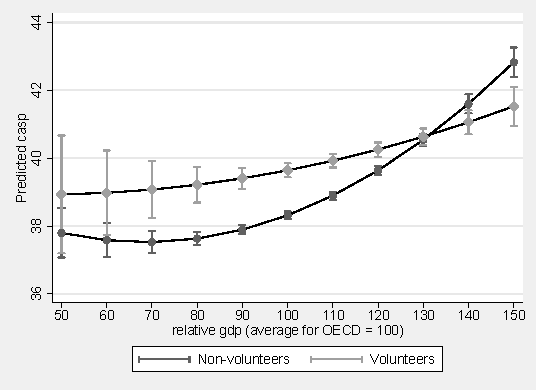
\includegraphics[height=2.7in]{pooling.pdf}}\quad
\subfloat[Change in predictive casp]{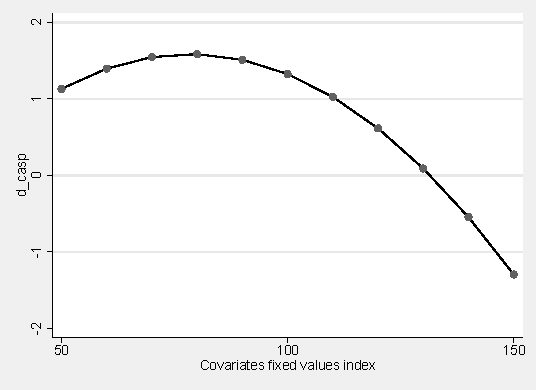
\includegraphics[height=2.7in]{d_casp_pooling.pdf}}~\\

\end{minipage}
\end{figure}


[{\bf TODO:} rephraze this chunk here] 
The results are consistent with the previouse finding on nonlinear effect of economic development on an impact of volunteering on QoL. We find higher effect in Italy, Greece, Isreal than in Poland, Denmark and Switzerland. This  is consistent with \citet{haski09} and with unconditional analysis with the Kendall's correlations. This is not very suprising since we do not control for differences in within group characteristics. So far, we know that volunteers have higher QoL but we do not know whether it is becouse they are active as volunteers or becouse they are generally have higher QoL. Positive estmiates on volunteering variable suggests that volunteering does have positive impact on QoL. In order to see how strong is that effect and whether it is different among countries we apply Juhn-Murphy-Pierce decomposition. 

\subsection*{Decomposition into endowment and price effect (JMP)}

Suppose that casp for volunteers and non-volunteers can be expressed by two separate equations:

  \begin{eqnarray}
	casp_{vi}= X_{vi}\beta_{vi}+ \epsilon_{vi}
 \end{eqnarray}
where $v=\big\{0,1\big\}$ denotes volunteers and non-volunteers, respectively. $X_{i}$ includes exogenous variables and $\beta_{i}$ is a vector of estimates of the casp equation. The stochastic component $\epsilon_{vi}$ is distributed with a mean zero and a variance of $\sigma_{vi}^{2}$. Let $F_{0}()$ and $F_{1}()$ denote  the cumulative distributions functions of the residuls for the separate models and $F()$ denotes the function for the whole sample. Then the pooled model is:  

  \begin{eqnarray}
	casp_{i}= X_{i}\beta+ F^{-1}(p_{i}|X_{i})
 \end{eqnarray}

where $F^{-1}(.)$ is the inverse of the cumulative distribution function. Assuming that $\beta_{0}=\beta_{1}$ we may calculate hypothetical outcomes that would have occured if the "prices" had been the same in both groups:

  \begin{eqnarray} 
	casp^{H}_{1i}= X_{1i}\beta+ F^{-1}(p_{1i}|X_{1i}) \label{eq:1} \\
	casp^{H}_{0i}= X_{0i}\beta+ F^{-1}(p_{0i}|X_{0i}) \label{eq:2}
 \end{eqnarray}

Let equation \ref{eq:1} denote as $casp^{H}_{1i}(\beta,F|X_{1i})$ and equation \ref{eq:2} denote as $casp^{H}_{0i}(\beta,F|X_{0i})$. Also, we may define $casp^{H}_{vi}(F|\beta_{v},X_{vi})$ where quantities $X$ and prices $ \beta_{v}$ are different but the residual distributions are the same. Then, we may define $ casp_{vi}(\beta_{v},F_{v})$ that denotes the original values. For those we use just short notation  $casp_{vi}$.
Let notice that:

\begin{enumerate}

\item  $ E(X_{1},X_{0})=\bigg[E[casp^{H}_{1}(\beta,F)|X_{1}]-E[casp^{H}_{0}(\beta,F)|X_{0}\bigg]$ is the difference in expected casp due to different endowments in variables included in X. We call it the endowment effect. 

\item $ V(\beta_{0},\beta_{1}) =\bigg[ [E[casp^{H}_{1}(F|\beta_{1},X_{1i})]- E[casp^{H}_{0}(F|\beta_{0},X_{1i})]] -E(X_{1},X_{0})\bigg]$ is the difference in the expected casp due to different valuations of variables in X. We call it "volunteering effect"

\item $ V(F_{0},F_{1}) =\bigg[ [E[casp_{1}]-E[casp_{0}]] - [E[casp^{H}_{1}(F|\beta_{1},X_{1i})]- E[casp^{H}_{0}(F|\beta_{0},X_{1i})]] \bigg] $ is the difference caused by differences in unobservables. We will call it "unobservables effect".

\end{enumerate}

Finally  we may write:
  \begin{eqnarray} 
	E[casp_{1}]-E[casp_{0}]= E(X_{1},X_{0}) +  V(\beta_{0},\beta_{1}) +  V(F_{0},F_{1})
 \end{eqnarray}


The three components are presented below:


\begin{figure}[H]
\centering
\caption{JMP Decomposition.} 
\label{fig:pooling1}
\begin{minipage}{1\linewidth}
\subfloat[JMP decomposition]{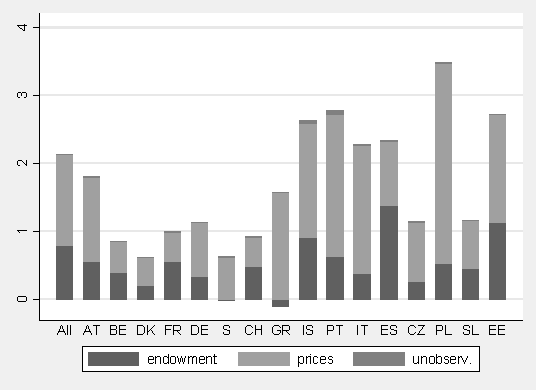
\includegraphics[height=2.7in]{ols_margins.pdf}}\quad
\subfloat[Volunteering effect (price) on casp. ]{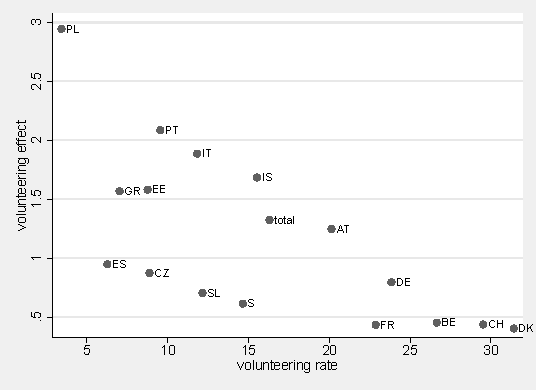
\includegraphics[height=2.7in]{vol_margins.pdf}}~\\

\end{minipage}
\end{figure}
 
Volunteers have higher level of quality of life. Part of the difference between them and non-volunteers can be explained by the differnces in socio-economic characteristcs and other characteristics that were not observed in the data. Panel a) of figure \ref{fig:pooling1} shows decomposition. Sums of the endowment effects and the unobservables effects are not very different across countries. Two exceptions are Greece and Sweden were those effects are smaller than in other countries. Taking into account those factors that are not directly related to volunteering does not change the main result. We conclude that impact of volunteering on individual QoL is higher in countries where volunteering is relatievly less popular. However, country specific factors are possible reasons for significant heterogenity among countries with low volunteering rates. Poland, Czech Republic and Estonia present the intresting case for the comparison in the future.   
 
\section{Discussion}

We used data from the wave 6 of the SHARE survey to study an association of volunteering with QoL. We calculated the Kendall tau-b correlation coefficients and compared  our results with those discussed in \citet{haski09}. We found the highest impact of volunteering on QoL in countries with mid-range values of the volunteering rates - Italy, Isreal, Austria. In countries with the high rates (Denmark, Switzerland, Belgium) and in countries with low rates (Poland, Greece, Czech Rep., Spain) that impact was lower. This confirmed Haski's finding about non-linear relation between impact of volunteering on QoL and economic development. 
In the second part of the paper we applied a multivariate analysis to check whether non-random selection into volunteering may be responsible for the above finding. Firstly, we showed that economic development positively influences the popularity of volunteering among elderly. In better developed countries we should expect to see larger fractions pf elderly involved in volunteering. Secondly, we showed that voluteers and non-volunteers differ in socio-economic characteristics within countries as well as between countries. The positive role of tertiary education was the only consistently significant factor for all countries. Two other variables that were significant in majority of countries were: income and health. Household and family based variables such as number of people living together in a household and number of grandchildren had a limited influence on choosing volunteering. The positive role of education and income makes us to expect higher QoL among volunteers than among non-volunteers even if those from the second group had not been involved into volunteering. Not taking into account diffrences in characteristics between volunteers and non-volunteers leads to the overestimation of the impact of voluntering on QoL since volunteers are recruited from people whose characteristics are positivly correlated with QoL. That is why we decomposed the mean difference in QoL conditional on volunteering into two elements. The first one measured the role of differences in socioeconmic variables and second one measured the  volunteering effect on QoL. Thirdly, thanks to such decomposition we showed that after controlling for the differences in endowment in socioeconomic factors the relation between  volunteering and its impact on QoL is more linear with higher impact among low rate countries and lower impact among high rate countries. This is consistent with the statment in \citet{plagnol10} that stresses the role of selection into the volunteering sector:

\begin{quote}
" ... volunteers in countries with a low frequency of volunteering displayed higher values on several of the wellbeing measures than those in other countries. (...) in countries where volunteering is generally less common, those who do participate in formal or informal volunteering have the highest levels of well-being. It may be that in these countries, only those who are most likely to benefit from volunteering actually volunteer. 
\end{quote}

Also, the work of \textbf{Thoits and Hewitt (2001), Li and Ferraro (2005), and Hao (2008)} documented that older adults with higher levels of well-being volunteer more (from Morrow-Howell 2010).

We found a strong support for our first hypothesis stating that there is significant variability among countries in a way how volunteering influences QoL.  Our results are in line with the previouse studies (\citet{haski09}, \citet{plagnol10}). We did not find the clear answer for the second hypothesis. We are likely to agree that volunteering has rather weak effect in countries with high rates. We think that the explanation given in \citet{haski09} stressing the role of feelings of necessity is the valid one.\footnote{\citet{haski09} wrote "(...) in countries where the welfare system is strong such as in Northern Europe, people volunteer more due to a stronger sense of solidarity,but perhaps feel less needed—if they will not deliver the services, the state or someone else would. Feelings of necessity are very important in creating satisfaction and attitudinal commitment among volunteers (Cnaan and Cascio 1999) and that may explain why the correlation between volunteering and wellbeing was weaker in these countries."}. It is possible that some social public expenditure might crowd out the private time donation. Bredtmann (2016) noticed that in order to reach such  conlcusion, we have to have clear understanding of the choice process leading to volunteering. If people treat government spendig as a near perfect substitute for own activity then the crowding will take place. If the volunteering decision is idependent on government spending than the crowding out should not be observed. The weak relation between vounteering and quality of life among highly developed countries in Europe does not allow us to reject the preasumption about too strong govermental support. Crowding out among elderly is not well recognized. It was discussed in relation to volunteering in general - for example \textbf{Hackl at al. (2016)}, \textbf{Stadelmann-Steffen (2011)} -  but we are not aware of any work on crowding out among elderly. The issue has important practical consequences so it should be discussed in future research.     

The crowding-out issue has rather minor significance in countries where the welfare state is weak. In these countries  volunteering among elderly is much more heterogenous. This suggests the bigger role for country specific cultural and historical factors. It may be also that the less developed  institutional framework makes costs of enagaging in volunteering higher in countries with weaker welfare system. This opens a possibility for efficiency enchancing state intervation. Demographic ageing and improvements of  health among elderly explain why public actions targeted in lowering costs of volunteering can bring noticable gain for society. Such actions make sense since number of people who reach their ‘third age’ without severe physical or mental impairment has been increasing. These people may continue their life by  engaging in productive activities with benefit for themselves for others. If the two main economic barriers--poor health and low income--have been losing their strength it is time for governments to take active role in promoting volunteering among volunteers. This might be especially important for countries in Central and Eastern Europe where the current rates of volunteering are low. [{\bf TODO:} rephraze past few sentences]

According to \textbf{Durlauf and Fafchamps (2005, p. 1648)} collective action can be treaed as substitute for the state. Voluntary activities may efficiently replace a state in delivering some public good. It may be cost efficient for the state to built a necessary organizational structure for the promotion of voluntary work than to purchase some services. Also, volunteering adds to social capital what has a positive impact on society well-being.  


\begin{thebibliography}{87}
\newcommand{\enquote}[1]{``#1''}
\expandafter\ifx\csname natexlab\endcsname\relax\def\natexlab#1{#1}\fi

\bibitem[\protect\citeauthoryear{Anderson, Damianakis, Kr{\"o}ger, Wagner, Dawson, Binns, Bernstein, Caspi, and Cook}{Anderson et~al.}{2014}]{anderson14}
\textsc{Anderson, N.~D., T.~Damianakis, E.~Kr{\"o}ger, L.~M. Wagner, D.~R.Dawson, M.~A. Binns, S.~Bernstein, E.~Caspi, and S.~L. Cook} (2014):  \enquote{The benefits associated with volunteering among seniors: a critical  review and recommendations for future research.} \emph{Psychological bulletin}, 140, 1505.

\bibitem[\protect\citeauthoryear{Bergmann, Kneip, De Luca, and Scherpenzeel}{Bergmann et~al.}{2017}]{bergmann17}
\textsc{Bergmann, M., T.~Kneip, G.~De Luca, A.~Scherpenzeel} (2017):  \enquote{Survey participation in the Survey of Health, Ageing and Retirement in Europe (SHARE), Wave 1-6.} \emph{Working Paper Series}, 31-2017.


\bibitem[\protect\citeauthoryear{Borgonovi}{Borgonovi}{2008}]{borgonovi08}
\textsc{Borgonovi, F.} (2008): \enquote{Doing well by doing good. The relationship between formal volunteering and self$-$reported health and happiness,} \emph{Social Science and Medicine}, 66,  2321 -- 2334.

\bibitem[\protect\citeauthoryear{Borrat-Besson, Ryser and Gonçalves}{Borrat-Besson et~al.}{2015}]{borrat15}
\textsc{Borrat-Besson, C.,V-A.~Ryser, and J.~Gonçalves} (2015):  \enquote{What impact does it really have?} \emph{An evaluation of the CASP-12 scale used in the Survey of Health, Ageing and Retirement in Europe (SHARE) to measure Quality of Life among people aged 50+}, \emph{FORS Working Papers}, 2015-4


\bibitem[\protect\citeauthoryear{Casiday, Kinsman, Fisher and Bambra}{Casiday et~al.}{2008}]{casiday08} 
\textsc{Casiday, R., E.~Kinsman, C.~Fisher and C.~Bambra} (2008):  \enquote{What impact does it really have?} \emph{Report to Volunteering England}, London: Volunteering England.

\bibitem[\protect\citeauthoryear{Detollenaere, Willems, Baert}{Detollenaere et~al.}{2017}]{detollenaere17}
\textsc{Detollenaere, J. and S.~Willems and S.~Baert} (2017): \enquote{Volunteering, income and health,} \emph{PLoS ONE}, 12(3):e0173139,  doi:10.1371/journal.pone.0173139.

\bibitem[\protect\citeauthoryear{Ehlers, Naegele, Reichert}{Ehers et~al.}{2011}]{ehlers11}
\textsc{Ehlers, A. and G.~Naegele and M.~Reichert} (2011): \enquote{Volunteering by older people in the EU,} \emph{European Foundation for the Improvement of Living and Working Conditions} 

Ehlers, Anja; Naegele, Gerhard; Reichert, Monika

\bibitem[\protect\citeauthoryear{Haski-Leventhal}{Haski-Leventhal}{2009}]{haski09}
\textsc{Haski-Leventhal, D.} (2009): \enquote{Elderly volunteering and
  well-being: A cross-European comparison based on SHARE data,} \emph{Voluntas:
  International Journal of Voluntary and Nonprofit Organizations}, 20, 388--404.
  
  % Potwierdzeni CASP in SHARE
%@article{doi:10.1080/13607863.2017.1292208,
%author = {Gema Pérez-Rojo and Noemy Martín and Cristina Noriega and Javier López},
%title = {Psychometric properties of the CASP-12 in a Spanish older community dwelling sample},
%journal = {Aging \& Mental Health},
%volume = {0},
%number = {0},
%pages = {1-9},
%year  = {2017},
%abstract = {Objective: Current studies have shown that older people's quality of life (QoL) is more associated to individual's sense of happiness and subjective life satisfaction than to objective problems. CASP scale conceptualizes QoL based on a psycho-sociological perspective. Originally, CASP consisted of 19 items (four factors: Control, Autonomy, Self-realization and Pleasure). Later, it was proposed a shorter version (12 items and three factors). The aim of this study was to assess the structure of the CASP-12 SHARE version using confirmatory factor analysis.  
  
\bibitem[\protect\citeauthoryear{Hank and Erlinghagen}{Hank and   Erlinghagen}{2009}]{hank09}
\textsc{Hank, K. and M.~Erlinghagen} (2009): \enquote{Dynamics of volunteering in older Europeans,} \emph{The Gerontologist}, 50, 170--178.  

\bibitem[\protect\citeauthoryear{Hyde}{Hyde}{2003}]{hyde03}
\textsc{Hyde, M.} (2003): \enquote{A measure of quality of life in early old age: The theory, development and properties of a needs satisfaction model (CASP-19),} \emph{Aging and mental health}, 7(3), 186--194. 


\bibitem[\protect\citeauthoryear{Jenkinson, Dickens, Jones, Thompson-Coon, Taylor, Rogers, Bambra, Lang, and Richards}{Jenkinson et~al.}{2013}]{jenkinson2013volunteering}
\textsc{Jenkinson, C.~E., A.~P. Dickens, K.~Jones, J.~Thompson-Coon, R.~S.Taylor, M.~Rogers, C.~L. Bambra, I.~Lang, and S.~H. Richards} (2013):
  \enquote{Is volunteering a public health intervention? A systematic review and meta-analysis of the health and survival of volunteers,} \emph{BMC public health}, 13, 773.

% Khamis H. Measures of Association: How to Choose? Journal of Diagnostic Medical Sonography. 2008;24:155-162.}

\bibitem[\protect\citeauthoryear{Li and Ferraro}{Li and Ferraro}{2006}]{li06}
\textsc{Li, Y. and KF.~Ferraro} (2006): \enquote{Volunteering in middle and later life: is health a benefit, barrier or both ?} \emph{Social Forces}, 85, 497--519. 


\bibitem[\protect\citeauthoryear{Meier and Stutzer}{Meier and
  Stutzer}{2008{\natexlab{b}}}]{meier08}
---\hspace{-.1pt}---\hspace{-.1pt}--- (2008{\natexlab{b}}): \enquote{Is volunteering rewarding in itself?} \emph{Economica}, 75, 39--59.

\bibitem[\protect\citeauthoryear{Morrow-Howell}{Morrow-Howell}{2010}]{morrow10}
\textsc{Morrow-Howell, N.} (2010):
  \enquote{Volunteering in later life: research frontiers} \emph{The Journals of Gerontology: Series B},65B(4), 461–469


\bibitem[\protect\citeauthoryear{Morrow-Howell, Hinterlong, Rozario and Tang}{Morrow-Howell et~al.}{2003}]{morrow2003}
\textsc{Morrow-Howell, N., J.~Hinterlong, P.~A.Rozario, F.~Tang} (2003):
  \enquote{Effects of Volunteering on the Well-Being of Older Adults,} \emph{The Journals of Gerontology: Series B},58, S137--S145

\bibitem[\protect\citeauthoryear{National Research Council (US) Panel on a Research Agenda and New Data for an Aging World}{National Research Council (US)}{2001}]{nrc2001}
\textsc{National Research Council (US) Panel on a Research Agenda and New Data for an Aging World)} (2001):
  \enquote{Preparing for an Aging World: The Case for Cross-National Research. ,} \emph{Washington (DC): National Academies Press (US)},2001, Available from: https://www.ncbi.nlm.nih.gov/books/NBK98384/


\bibitem[\protect\citeauthoryear{Oecd}{Oecd}{2015}]{Oecd15}
\textsc{Oecd} (2015): \enquote{How's Life  2015 - Measuring Well-being} \emph{OECD 2015}.

\bibitem[\protect\citeauthoryear{Oecd}{Oecd}{2016}]{Oecd16}
\textsc{Oecd} (2016): \enquote{Society at Glance} \emph{OECD 2016}.

 \bibitem[\protect\citeauthoryear{Plagnol and Huppert}{Plagnol and Huppert}{2010}]{plagnol10}
\textsc{Plagnol, A. C. and ~F-A.Huppert } (2010): \enquote{Happy to help? Exploring the factors associated with variations in rates of volunteering across Europe,} \emph{Social Indicators Research}, 97(2), 157--176.
  
 \bibitem[\protect\citeauthoryear{Prouteau and Wolff}{Prouteau and Wolff}{2006}]{prouteau06}
\textsc{Prouteau, L. and ~F-C.Wolff } (2006): \enquote{Does volunteer work pay off in the labor market?,} \emph{Journal of Socio-Economics}, 35, 992--1013.

\bibitem[\protect\citeauthoryear{Salamon, Haddock, and Sokolowski}{Salamon et~al.}{2017}]{salomon2017} \textsc{Salamon, L.~M., M.~A. Haddock and W.~S. Sokolowski}(2017):
 \enquote{Closing the Gap? New Perspectives on Volunteering North and South,} \emph{J. Butcher, C.J. Einolf (eds.), Perspectives on Volunteering, Nonprofit and Civil Society Studies, $DOI 10.1007/978-3-319-39899-0_2$}, chapter 2, 29--51.
  
\bibitem[\protect\citeauthoryear{Thoits and Hewitt}{Thoits and Hewitt}{2001}]{thoits03}
\textsc{Thoits, P.A. and ~L.N.Hewitt } (2001): \enquote{Volunteer Work and Well-Being,} \emph{Volunteer Work and Well-Being},42, 115--131.


\bibitem[\protect\citeauthoryear{Whillans, Seider, Chen, Dwyer, Novick, Gramign, Mitchell, Savalei, Dickerson and Dunn}{Whillans et~al.}{2016}]{whillans2016}
\textsc{Whillans, A.~V., S.~C. Seider, L.~Chen, R.~J. Dwyer, S.~Novick, K.~J.Gramign, B.~A. Mitchell, V.~Savalei, S.~S.Dickerson and E.~W. Dunn}(2016):
  \enquote{Does volunteering improve well-being?,} \emph{omprehensive Results in Social Psychology}, 1, 35--50.

  
\bibitem[\protect\citeauthoryear{Wilson}{Wilson}{2012}]{wilson12}
\textsc{Wilson, J.} (2012): \enquote{Volunteerism research: A
  review essay,} \emph{Nonprofit and Voluntary Sector Quarterly}, 41, 176--212.

\bibitem[\protect\citeauthoryear{Ziemek}{Ziemek}{2006}]{ziemek06}
\textsc{Ziemek, S.} (2006): \enquote{Economic analysis of volunteers` motivations. A cross$-$country study,} \emph{Journal of Socio$-$Economics}, 35(3), 532--555.


\bibitem[\protect\citeauthoryear{Van Willigen}{Van Willigen}{2000}]{VanWilligen00}
\textsc{Van Willigen, M.} (2000): \enquote{Differential benefits of volunteering across the life course,} \emph{Journal of Gerontology Series B}, 55, 5308--5318.


\end{thebibliography}


\begin{spacing}{.9}

\section{Appendix: additional descriptive statistics}


%%%%%%%%%%%%%%%%%%%%%%%%%%%%%%%%%%%%%%%%%%%%%%%%%%%%%%%%%%%%%%%%
% Rozkład CASP
\begin{figure}[H]
 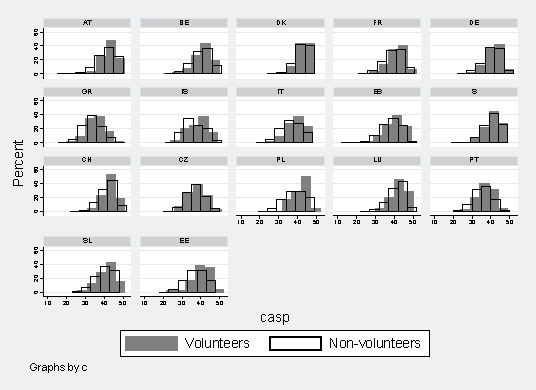
\includegraphics[height=3in]{hist_casp.pdf}
 \centering
 \label{fig:hist_casp}
\caption{Distribution of CASP by countries}
\end{figure}

%%% TABLE: Kendall tau-b
\begin{spacing}{.9}
	 % Table generated by Excel2LaTeX from sheet 'casp'
\begin{table}[htbp]
  \centering
  \caption{Significance test - Kendall tau correlations}
    \begin{tabular}{lrccccccccccccccccc}
          &       & IT    & AT    & EE    & FR    & LU    & DE    & SL    & SE    & BE    & PT    & PL    & CH    & CR    & GR    & DK    & CZ    & S \\
    IS    & 15.4 & 64.1 & 58.4 & 54.2 & 19.0 & 15.8 & \textbf{5.0} & \textbf{3.6} & \textbf{2.1} & \textbf{1.8} & \textbf{5.3} & \textbf{1.5} & \textbf{0.6} & \textbf{0.4} & \textbf{0.2} & \textbf{0.0} & \textbf{0.0} & \textbf{0.0} \\
    IT    & 14.4 & X     & 87.9 & 83.8 & 23.7 & 20.7 & \textbf{3.6} & \textbf{2.2} & \textbf{0.9} & \textbf{0.6} & \textbf{5.7} & \textbf{1.0} & \textbf{0.3} & \textbf{0.1} & \textbf{0.0} & \textbf{0.0} & \textbf{0.0} & \textbf{0.0} \\
    AT    & 14.1 &       & X     & 98.0 & 36.2 & 28.2 & \textbf{8.9} & \textbf{6.1} & \textbf{3.4} & \textbf{2.6} & \textbf{9.5} & \textbf{2.5} & \textbf{0.9} & \textbf{0.5} & \textbf{0.1} & \textbf{0.0} & \textbf{0.0} & \textbf{0.0} \\
    EE    & 14.1 &       &       & X     & 31.9 & 25.9 & \textbf{5.7} & \textbf{3.7} & \textbf{1.6} & \textbf{1.2} & \textbf{7.8} & \textbf{1.6} & \textbf{0.4} & \textbf{0.2} & \textbf{0.0} & \textbf{0.0} & \textbf{0.0} & \textbf{0.0} \\
    FR    & 12.3 &       &       &       & X     & 69.8 & 43.4 & 33.6 & 24.0 & 20.3 & 33.2 & 13.6 & \textbf{6.7} & \textbf{4.4} & \textbf{2.2} & \textbf{0.2} & \textbf{0.0} & \textbf{0.0} \\
    LU    & 11.4 &       &       &       &       & X     & 85.5 & 74.9 & 65.6 & 60.6 & 63.6 & 39.6 & 28.6 & 22.9 & 19.7 & \textbf{4.9} & \textbf{1.3} & \textbf{0.1} \\
    DE    & 10.9 &       &       &       &       &       & X     & 84.7 & 71.1 & 63.6 & 69.2 & 38.0 & 23.8 & 17.3 & 11.7 & \textbf{1.5} & \textbf{0.1} & \textbf{0.0} \\
    SL    & 10.6 &       &       &       &       &       &       & X     & 87.0 & 79.1 & 80.1 & 47.3 & 31.5 & 23.6 & 17.5 & \textbf{2.5} & \textbf{0.3} & \textbf{0.0} \\
    SE    & 10.3 &       &       &       &       &       &       &       & X     & 91.4 & 88.7 & 53.8 & 36.2 & 27.2 & 20.1 & \textbf{2.7} & \textbf{0.2} & \textbf{0.0} \\
    BE    & 10.1 &       &       &       &       &       &       &       &       & X     & 94.5 & 59.3 & 41.0 & 31.2 & 24.1 & \textbf{3.5} & \textbf{0.3} & \textbf{0.0} \\
    PT    & 10.0 &       &       &       &       &       &       &       &       &       & X     & 72.2 & 57.8 & 48.9 & 45.9 & 14.5 & \textbf{4.8} & \textbf{0.6} \\
    PL    & 9.0 &       &       &       &       &       &       &       &       &       &       & X     & 84.3 & 73.2 & 71.4 & 24.6 & \textbf{8.5} & \textbf{1.1} \\
    CH    & 8.6 &       &       &       &       &       &       &       &       &       &       &       & X     & 87.9 & 87.5 & 30.9 & 10.5 & \textbf{1.2} \\
    CR    & 8.2 &       &       &       &       &       &       &       &       &       &       &       &       & X     & 98.9 & 38.7 & 14.3 & \textbf{1.8} \\
    GR    & 8.2 &       &       &       &       &       &       &       &       &       &       &       &       &       & X     & 31.6 & \textbf{8.7} & \textbf{0.6} \\
    DK    & 6.4 &       &       &       &       &       &       &       &       &       &       &       &       &       &       & X     & 54.6 & 10.9 \\
    CZ    & 5.3 &       &       &       &       &       &       &       &       &       &       &       &       &       &       &       & X     & 28.1 \\
    S     & 3.3 &       &       &       &       &       &       &       &       &       &       &       &       &       &       &       &       & X \\
    \end{tabular}%
  \label{tab:addlabel}%
\end{table}%

      \label{KendallCasp} 
\end{spacing}
%%%% END: TABLE



%%%%%%%%%%%%%%%%%%%  DESCRIPTIVES %%%%%%%%%%%%%%%%%%%%%%%%%

 

% Age distribution
\begin{figure}[H]
 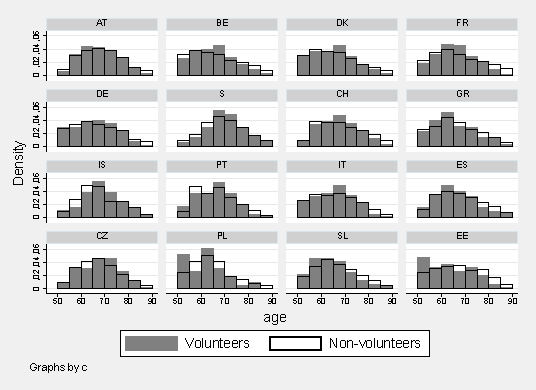
\includegraphics[height=3in]{hist_age.pdf}
 \centering
 \label{fig:hist_age}
\caption{Age distribution}
\end{figure}


%%% TABLE
\begin{spacing}{.9}
\centering 
\begin{scriptsize} 
	 \begin{table}[htbp]\centering
\def\sym#1{\ifmmode^{#1}\else\(^{#1}\)\fi}
\caption{Non-volunteers}
\begin{tabular}{l*{4}{c}}
\hline\hline
            &\multicolumn{4}{c}{(1)}                            \\
            &\multicolumn{4}{c}{}                               \\
            &           1&           2&           3&           4\\
            &      rowpct&      rowpct&      rowpct&      rowpct\\
\hline
AT          &       10.20&       12.40&       52.33&       25.06\\
BE          &       15.75&       22.32&       28.51&       33.41\\
DK          &        7.96&        9.36&       40.81&       41.87\\
FR          &       32.12&        8.70&       37.92&       21.26\\
DE          &        0.77&        9.32&       57.54&       32.37\\
GR          &       37.68&       10.54&       29.59&       22.20\\
IS          &       19.51&        9.32&       34.95&       36.21\\
IT          &       38.79&       28.44&       23.70&        9.06\\
ES          &       53.47&       23.67&       12.01&       10.85\\
S           &       20.16&       14.36&       33.97&       31.50\\
CH          &        9.40&        9.15&       66.20&       15.25\\
CZ          &       10.39&       26.60&       49.37&       13.64\\
PL          &       23.97&        4.21&       61.24&       10.58\\
LU          &       32.51&       11.15&       40.61&       15.73\\
PT          &       52.57&        8.33&        7.72&       31.37\\
SL          &        6.89&       21.89&       53.64&       17.58\\
EE          &        2.60&       19.02&       52.40&       25.98\\
\hline\hline
\end{tabular}
\end{table}
\begin{table}[htbp]\centering
\def\sym#1{\ifmmode^{#1}\else\(^{#1}\)\fi}
\caption{Volunteers}
\begin{tabular}{l*{4}{c}}
\hline\hline
            &\multicolumn{4}{c}{(1)}                            \\
            &\multicolumn{4}{c}{}                               \\
            &           1&           2&           3&           4\\
            &      rowpct&      rowpct&      rowpct&      rowpct\\
\hline
AT          &        4.54&        9.98&       49.18&       36.30\\
BE          &        7.45&       17.99&       25.94&       48.62\\
DK          &        5.94&        6.34&       34.74&       52.97\\
FR          &       15.77&        5.69&       39.85&       38.69\\
DE          &        0.00&        6.61&       53.36&       40.02\\
GR          &       32.05&       11.58&       27.03&       29.34\\
IS          &        9.79&        6.70&       35.05&       48.45\\
IT          &       23.61&       27.68&       35.84&       12.88\\
ES          &       28.20&       19.17&       22.56&       30.08\\
S           &       18.53&       11.16&       33.47&       36.84\\
CH          &        5.84&        8.32&       62.34&       23.50\\
CZ          &        4.80&       14.41&       49.44&       31.36\\
PL          &        4.35&        0.00&       58.70&       36.96\\
LU          &       16.14&        9.49&       46.84&       27.53\\
PT          &       23.76&       14.85&        8.91&       52.48\\
SL          &        2.29&       15.33&       54.69&       27.69\\
EE          &        0.28&        9.09&       38.92&       51.70\\
\hline\hline
\end{tabular}
\end{table}

      \label{StatEdu} 
\end{scriptsize}
\end{spacing}
%%%% END: TABLE


%%% TABLE
\begin{spacing}{.9}
\centering 
\begin{scriptsize} 
	 {
\def\sym#1{\ifmmode^{#1}\else\(^{#1}\)\fi}
\begin{tabular}{l*{4}{c}}
\hline\hline
            &\multicolumn{4}{c}{(1)}                            \\
            &\multicolumn{4}{c}{}                               \\
            &           2&           3&           4&           5\\
            &      rowpct&      rowpct&      rowpct&      rowpct\\
\hline
AT          &       34.39&       39.42&       24.14&        2.05\\
BE          &       31.43&       50.45&       16.34&        1.77\\
DK          &       59.34&       22.61&       15.24&        2.81\\
FR          &       24.41&       47.22&       23.41&        4.95\\
DE          &       20.42&       46.17&       29.00&        4.41\\
S           &       44.24&       35.64&       17.95&        2.18\\
CH          &       39.77&       44.16&       13.98&        2.10\\
GR          &       39.32&       39.19&       19.11&        2.38\\
IS          &       46.60&       31.17&       18.83&        3.40\\
PT          &       10.66&       32.97&       49.02&        7.35\\
IT          &       26.64&       42.66&       28.25&        2.45\\
ES          &       26.86&       46.88&       22.57&        3.68\\
CZ          &       18.77&       42.41&       32.08&        6.75\\
PL          &       11.61&       46.35&       32.68&        9.36\\
SL          &       18.07&       49.96&       25.87&        6.10\\
EE          &        6.60&       27.75&       56.61&        9.04\\
\hline\hline
\end{tabular}
}
{
\def\sym#1{\ifmmode^{#1}\else\(^{#1}\)\fi}
\begin{tabular}{l*{4}{c}}
\hline\hline
            &\multicolumn{4}{c}{(1)}                            \\
            &\multicolumn{4}{c}{}                               \\
            &           2&           3&           4&           5\\
            &      rowpct&      rowpct&      rowpct&      rowpct\\
\hline
AT          &       48.64&       37.02&       13.25&        1.09\\
BE          &       40.59&       46.61&       12.13&        0.67\\
DK          &       67.77&       20.24&       10.17&        1.81\\
FR          &       31.09&       49.78&       16.50&        2.63\\
DE          &       28.14&       43.39&       26.46&        2.02\\
S           &       45.68&       34.32&       17.68&        2.32\\
CH          &       50.51&       42.34&        6.57&        0.58\\
GR          &       43.24&       33.98&       18.53&        4.25\\
IS          &       47.94&       26.29&       24.74&        1.03\\
PT          &       15.84&       34.65&       42.57&        6.93\\
IT          &       29.18&       48.71&       19.96&        2.15\\
ES          &       30.45&       52.26&       15.04&        2.26\\
CZ          &       30.23&       39.83&       26.84&        3.11\\
PL          &       15.22&       58.70&       23.91&        2.17\\
SL          &       22.43&       49.89&       23.34&        4.35\\
EE          &       17.05&       38.07&       40.91&        3.98\\
\hline\hline
\end{tabular}
}

      \label{StatHealth} 
\end{scriptsize}
\end{spacing}
%%%% END: TABLE


\begin{figure}[H]
\centering
\caption{Income and volunteering} 
\label{fig:casp_ols}
\begin{minipage}{1\linewidth}
\subfloat[Southern and Central Europe]{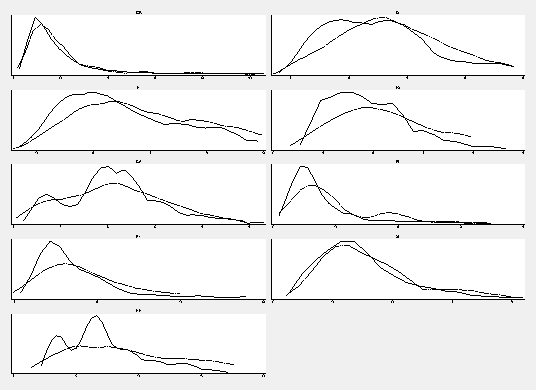
\includegraphics[height=2.7in]{hist_incCEE.pdf}}\quad
\subfloat[Western Europe]{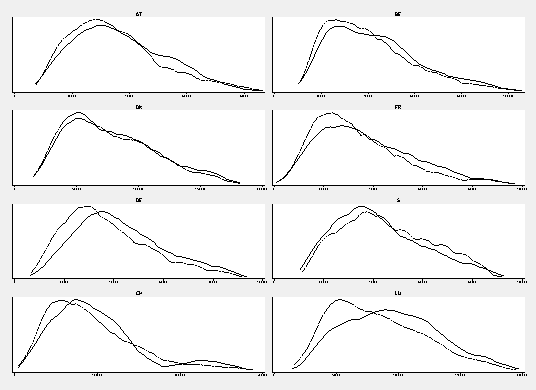
\includegraphics[height=2.7in]{hist_incWE.pdf}}~\\ 
{\footnotesize Notes: }~\\
{\footnotesize Source: Own calculations based on SHARE Wave 6.}
\end{minipage}
\end{figure} 

%%%%%%%%%%%%%%%%%%  TAU %%%%%%%%%%%%%%%%%%%%%%%%%

%%%% TABLE
%\begin{spacing}{.9}
%	 % Table generated by Excel2LaTeX from sheet 'Health'
\begin{table}[H]
  \centering
  \caption{Volunteering and health (taub): pvalues}
    \begin{tabular}{lrrrrrrrrrrrrr}
          & \multicolumn{1}{c}{AT} & \multicolumn{1}{c}{FR} & \multicolumn{1}{c}{BE} & \multicolumn{1}{c}{CH} & \multicolumn{1}{c}{DE} & \multicolumn{1}{c}{DK} & \multicolumn{1}{c}{CZ} & \multicolumn{1}{c}{IT} & \multicolumn{1}{c}{SE} & \multicolumn{1}{c}{PL} & \multicolumn{1}{c}{IS} & \multicolumn{1}{c}{GR} & \multicolumn{1}{c}{S} \\
          & \multicolumn{1}{c}{0.201} & \multicolumn{1}{c}{0.229} & \multicolumn{1}{c}{0.266} & \multicolumn{1}{c}{0.295} & \multicolumn{1}{c}{0.239} & \multicolumn{1}{c}{0.314} & \multicolumn{1}{c}{0.089} & \multicolumn{1}{c}{0.118} & \multicolumn{1}{c}{0.147} & \multicolumn{1}{c}{0.034} & \multicolumn{1}{c}{0.155} & \multicolumn{1}{c}{0.07} & \multicolumn{1}{c}{0.063} \\
          & \multicolumn{1}{c}{-0.162} & \multicolumn{1}{c}{-0.125} & \multicolumn{1}{c}{-0.123} & \multicolumn{1}{c}{-0.121} & \multicolumn{1}{c}{-0.112} & \multicolumn{1}{c}{-0.099} & \multicolumn{1}{c}{-0.085} & \multicolumn{1}{c}{-0.082} & \multicolumn{1}{c}{-0.081} & \multicolumn{1}{c}{-0.073} & \multicolumn{1}{c}{-0.04} & \multicolumn{1}{c}{-0.021} & \multicolumn{1}{c}{-0.017} \\
    AT    &       &       &       &       &       &       &       &       &       &       &       &       &  \\
    FR    & 0.079 &       &       &       &       &       &       &       &       &       &       &       &  \\
    BE    & 0.045 & 0.904 &       &       &       &       &       &       &       &       &       &       &  \\
    CH    & 0.071 & 0.845 & 0.92  &       &       &       &       &       &       &       &       &       &  \\
    DE    & 0.015 & 0.497 & 0.539 & 0.675 &       &       &       &       &       &       &       &       &  \\
    DK    & 0.003 & 0.202 & 0.208 & 0.33  & 0.528 &       &       &       &       &       &       &       &  \\
    CZ    & 0     & 0.041 & 0.036 & 0.098 & 0.168 & 0.49  &       &       &       &       &       &       &  \\
    IT    & 0     & 0.022 & 0.017 & 0.064 & 0.108 & 0.38  & 0.864 &       &       &       &       &       &  \\
    SE    & 0     & 0.017 & 0.013 & 0.053 & 0.09  & 0.341 & 0.811 & 0.946 &       &       &       &       &  \\
    PL    & 0     & 0.029 & 0.027 & 0.061 & 0.101 & 0.283 & 0.601 & 0.688 & 0.723 &       &       &       &  \\
    IS    & 0     & 0.001 & 0.001 & 0.003 & 0.005 & 0.025 & 0.076 & 0.091 & 0.098 & 0.258 &       &       &  \\
    GR    & 0     & 0     & 0     & 0     & 0     & 0     & 0.001 & 0.001 & 0.001 & 0.027 & 0.446 &       &  \\
    S     & 0     & 0     & 0     & 0     & 0     & 0     & 0.001 & 0.001 & 0.001 & 0.022 & 0.383 & 0.864 &  \\
    \end{tabular}%
  \label{tab:addlabel}%
\end{table}%

%      \label{tauH} 
%\end{spacing}
%%%%% END: TABLE

%%% TABLE
%\begin{spacing}{.9}
%	 \begin{table}[htbp]\centering
\def\sym#1{\ifmmode^{#1}\else\(^{#1}\)\fi}
\caption{Kandall tau-b (casp)}
\begin{tabular}{l*{1}{ccc}}
\hline\hline
                    &\multicolumn{3}{c}{(1)}               \\
                    &\multicolumn{3}{c}{}                  \\
                    &          N1&   estimate1&        dof1\\
\hline
AT                  &       20.14&       14.10&        3082\\
DE                  &       23.85&       10.93&        4145\\
S                   &       14.65&        3.29&        3650\\
SE                  &        6.27&       10.32&        4868\\
IT                  &       11.83&       14.37&        4891\\
FR                  &       22.87&       12.34&        3595\\
DK                  &       31.42&        6.41&        3520\\
GR                  &        7.02&        8.24&        4636\\
CH                  &       29.53&        8.55&        2661\\
BE                  &       26.65&       10.15&        5329\\
IS                  &       15.53&       15.40&        1643\\
CZ                  &        8.88&        5.28&        4377\\
PL                  &        3.43&        9.03&        1697\\
LU                  &       24.75&       11.37&        1454\\
PT                  &        9.55&        9.99&        1452\\
SL                  &       12.15&       10.59&        3938\\
EE                  &        8.76&       14.05&        5018\\
\hline\hline
\end{tabular}
\end{table}

%      \label{KendallCasp} 
%\end{spacing}
%%%% END: TABLE




%\section{Statistical Appendix}
%
%Mean decomposition for a fixed-effect model \\
% \begin{eqnarray}
%	casp_{i,c}= \beta_{0c}+ \beta_{1c}*v_{i,c} + \gamma_{c}*Z_{i,c} + \epsilon_{i,c}
% \end{eqnarray}
%
%\[ E[casp_{c}|v_{i,c}=1]= \beta_{0c}+\beta_{1c} + \gamma_{c}*E[Z_{c}|v_{i,c}=1]=\beta_{0c}+\beta_{1c} + \gamma_{c}*\bar{Z}_{c}(1) \]	\\
%	
%\[	E[casp_{c}|v_{i,c}=0]= \beta_{0c}+ \gamma_{c}*E[Z_{c}|v_{i,c}=0]=\beta_{0c}+ \gamma_{c}*\bar{Z}_{c}(0) \] \\
%	
%\[	E[casp_{c}|v_{i,c}=1] - E[casp_{c}|v_{i,c}=0]= \beta_{1c}+ \gamma_{c}*[\bar{Z}_{c}(1)-\bar{Z}_{c}(0)]
%\] \\
%
%Mean decomposition for a random-effect model \\
%
% \begin{eqnarray}
%	casp_{i,c}=\beta_{0}+  \beta_{1c}(r_{c})* vol_{i,c}+\gamma*Z_{i,c} + \epsilon_{i,c} 
% \end{eqnarray}
%
%where: 
% \begin{eqnarray}
%		\beta_{1} \sim N(\gamma_{1r}ln(r_{c}),\sigma^{2}_{r})
% \end{eqnarray}
%
%$[E[casp_{c}|v_{i,c}=1]= \beta_{0}+E[\beta_{1}(r_{c})|v_{i,c}=1] + \gamma*E[Z_{c}|v_{i,c}=1]+ E[\epsilon_{i,c}|v_{i,c}=1]=$ \\
%\\
%$=\beta_{0}+ [\beta_{1}+u_{r}(c)]+\gamma*\bar{Z}_{c}(1) + \bar{\epsilon}_{i,c}(1) $
%\\ 
%  
%\[E[casp_{c}|v_{i,c}=0]= \beta_{0}+ \gamma*E[Z_{c}|v_{i,c}=0] + E[\epsilon_{i,c}|v_{i,c}=0] = \beta_{0}+  \gamma*\bar{Z}_{c}(0) + \bar{\epsilon}_{i,c}(0) \]
%
%\[E[casp_{c}|v_{i,c}=1]-E[casp_{c}|v_{i,c}=0]= [\beta_{1}+u_{r}(c)]+ \gamma*(\bar{Z}_{c}(1)-\bar{Z}_{c}(0))+ [\bar{\epsilon}_{i,c}(1)-\bar{\epsilon}_{i,c}(0)] \]

\end{spacing}
\end{spacing}
\end{document}
